% !Mode:: "TeX:UTF-8"
% !TEX program  = xelatex
\documentclass[withoutpreface,bwprint]{cumcmthesis}
\usepackage{gbt7714}
\usepackage{array}
\usepackage{booktabs}
\bibliographystyle{gbt7714-numerical}
\title{Hello Typeset}
\tihao{A}            % 题号
\baominghao{4321}    % 报名号
\schoolname{重庆邮电大学}
\membera{Peitsan}
\memberb{SY}
\memberc{LH}
\supervisor{BOSS}
\yearinput{2022}     % 年
\monthinput{09}      % 月
\dayinput{13}        % 日

\begin{document}
	\maketitle
	\begin{abstract}
		用到了模型方法,就XX进行研究,解决了XX实际问题`
		
		针对问题一, XXX使用XX,为了就XX问题进行了研究 问题一中,对XX问题,根据XX方法,建立了XX数学模型,得出XX结论:S113、S116、S205等50家供应商对移动公司最为重要,详见附录XX。
		
		针对问题二.....
		
		\\
		
		针对问题三,基于问题二中无人机编队的调整算法,我们考虑在此之上加以改进,使得对于锥形编队改进机队调整方案。同样的,通过\textbf{计算机模拟}生成的多组测试集。然后,引入\textbf{三点定位法}来先验检索无人机的坐标。通过\textbf{卡尔曼滤波器}进行机队位置的后验更新,每次无人机调整都调用一次“卡尔曼滤波”,使误差趋于最小,认为此时无人机到达标的位置。依照本方法,最终使15架无人机均可以到达图3所示的锥形编队位置。
		
		本文解决了XX实际问题,具有XX实际意义,还可以XX改进。
		
		\keywords{卡尔曼滤波\quad  计算机模拟\quad   无人机编队 关键词4\quad 关键词5\quad}
		%这里最好在关键词之间加个空格
	\end{abstract}
		\section{问题重述}
	\subsection{问题背景}
	
	
	%背景段落
	当今,无人机具有丰富的应用场景。为了迎合实际应用需求,常需使得无人机集群按一定姿态遂行编队飞行。为避免外界干扰,应尽量保持电磁静默,减少电磁波发射。“纯方位无源定位”法是一种实用的机队姿态稳定算法——该算法将机队成员赋予固定编号,由其中某几架无人机发射信号(简记为“发射机”)、其余无人机被动接收信号(简记为“接收机”);并约定“接收机"得到的方向信息为“相对方位角$\alpha$”,定义为参考无人机与任意两架“发射机”连线的夹角,如图1中$\alpha_{1}$、$\alpha_{2}$、$\alpha_{3}$所示:
	
	%保留题目要求的图片
	\begin{figure}[htbp!]
		\centering
		\captionsetup{font={small}}
		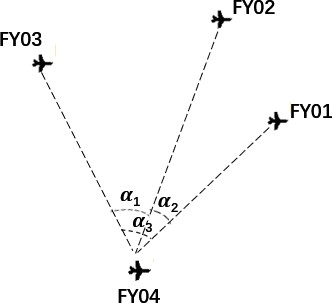
\includegraphics[height=4cm]{./figures/1-1.png}
		\caption{以FY04为参考机的相对方位角$\alpha$示例图}
		\label{fig:1}
	\end{figure}
	
	%排版图片时 应该相对集中 多幅图片在同一章节才能用多栏排版并排
	
	\subsection{问题提出}
	\begin{figure}[!htpb]
		\begin{minipage}{0.48\linewidth}
			\centering
			\captionsetup{font={small}}
			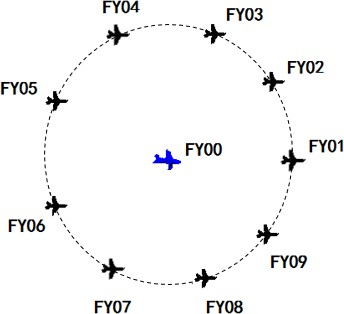
\includegraphics[height=4cm]{./figures/1-2.png}
			\caption{圆形无人机编队示意图}\label{fig:2}
		\end{minipage}
		\begin{minipage}{0.48\linewidth}
			\centering
			\captionsetup{font={small}}
			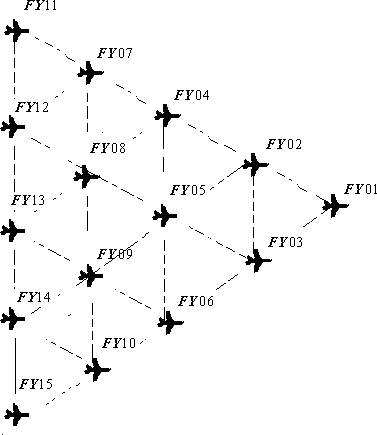
\includegraphics[height=4cm]{./figures/1-3.png}
			\caption{锥形无人机编队示意图}\label{fig:3}
		\end{minipage}
	\end{figure}	
	
	\noindent\textbf{问题一:}
	现有一组由10架有序无人机组成的圆形遂行机队,如图2所示,编号分别为FY01$\sim$FY09的成员机在以“FY00号无人机”为心的圆周上,依次解决下述问题:
	
	(1)编队中由包括“FY00号机”在内的3架无人机发射信号,其余偏移较大的成员为“接收机”,当已知“发射机”编号且位置无偏时,建立各“接收机”的定位模型。
	
	(2)假设“发射机”位置无偏差,已有FY00号和FY01号“发射机”时,还需要几架“发射机”才能实现“接收机”的有效定位。%编号未知
	
	(3)要求每次机队调整以“FY00号并另选3架无人机”作为“发射机”,其余作为“接收机”,仅根据表1中被选为“接收机”的方向信息,设计合理具体的无人机位置矫正方案,使外围的9架无人机最终均匀落在某半径为100 m的圆周上。
	
	%图1
	
	

	
	\noindent\textbf{问题二:}
	仍使用纯方位无源定位法,设计适合其他编队队形的位置调整方案,以如图3所示的锥形编队队形为例(间距均等于50m),阐述矫正方案设计过程。
	
	%		\begin{figure}[htbp!]
	%			\centering
	%			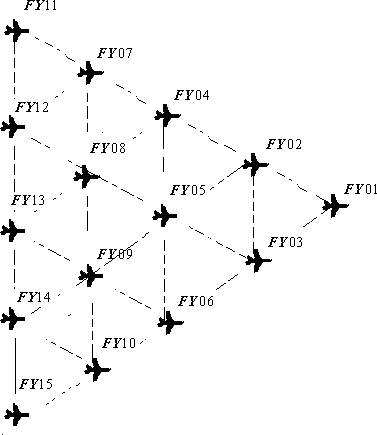
\includegraphics[width=6cm]{./figures/1-3.png}
	%			\caption{锥形无人机编队示意图}\label{fig:3}
	%		\end{figure}
	%		
		%表1
		
		%表格最好安排在章节的最后的位置 插在章节中间很丑
	\begin{table}[htbp!]
		\small
		\captionsetup{font={small}}
		\caption{无人机的初始位置}
		\centering
		\renewcommand\arraystretch{4}
		\tabcolsep=0.6cm
		\begin{tabular}{@{}cccc@{}}
			\toprule
			\textbf{无人机编号} & \textbf{极坐标 (m,\textdegree)} & \textbf{无人机编号} & \textbf{极坐标 (m,\textdegree)} \\ \midrule
			\textbf{0}     & (0, 0)             & \textbf{5}     & (98, 159.86)       \\
			\textbf{1}     & (100, 0)           & \textbf{6}     & (112, 199.96)      \\
			\textbf{2}     & (98, 40.10)        & \textbf{7}     & (105, 240.07)      \\
			\textbf{3}     & (112, 80.21)       & \textbf{8}     & (98, 280.17)       \\
			\textbf{4}     & (105, 119.75)      & \textbf{9}     & (112, 320.28)      \\ \bottomrule
		\end{tabular}
	\end{table}
	
	\section{模型的假设}
	
	(1)假设编队内各无人机均可根据自身感知的高度信息保持飞行在同一高度。
	
	(2)针对问题一前两种情况,假设“发射机”可以无偏差地稳定在圆周上,第三种情况下“发射机”有位置偏差。
	
	(3)假设编队内无人机位调整位置的时间忽略不计,视为“瞬间”完成位移。
	
	\section{符号说明}
	
	\begin{center}
		\small
		\captionsetup{font={small}}
		\renewcommand\arraystretch{3}
		\begin{tabular}{ccc}
			\hline
			\makebox[0.25\textwidth][c]{符号}	& \makebox[0.35\textwidth][c]{意义} & \makebox[0.2\textwidth][c]{单位}	 \\ \hline
			$\alpha$	    & 相对方向角 & \textdegree  \\ \hline
			$F_{i}$	    & 对应编号为FY0i的无人机的坐标点 &  -\\ \hline
			$\rho_{i}$	    & 编号为FY0i的无人机到FY00的距离 & m  \\ \hline
			$\theta_{i}$	    & 第i个夹角(按实际场景区分)& \textdegree  \\ \hline
			$Loss^{(t)}$ ,$Loss^{(A)}$	    &三角形队列、矩形队列模型的损失函数& -  \\ \hline	
			$P_{k}$	    & 第k次调整时的卡尔曼滤波协方差矩阵& 	-  \\ \hline
			$X_{k}$	    & 第k次调整时状态向量& - 	 \\ \hline
			$U_{k}$	    & 第k次调整时状态均值向量& - 	 \\ \hline
		\end{tabular}
		
	\end{center}
	\section{问题分析}
	
	\subsection{考虑“发射机”可以无偏差运行在圆周轨道上}
	
	问题一的情况(1)、(2)中,认为圆周上的发射机没用位置偏差,故可以对模型做简化,认为这两家发射机离圆心恒等于半径。同时,由于\textbf{外围无人机均匀排布}“”,便可理想认为任意相邻的两无人机夹角均为$\frac{\pi}{9}$;参照纯方位无缘定位方法,确定出2架“发射机”后,便依次易得各无人机方位角。
	,
	\subsection{考虑解析运算出代求接收机的方位信息}
	
	问题一(1)小问要求设计对“接收机”的定位模型,而确定“接收机”的方位需\textbf{计算方位角和极径长}。同时依题意,3架发射机无位置偏差且已知编号,基于4.1中的浅析,容易定位出各“接受机”的方位角。故本题需着重考虑各“接收机”到圆心的距离$L$。
	
	\subsection{考虑无人机定位方案进行优化校验}
	
	问题一(2)小问约定了除选FY00、FY01号外,另外确定一些无人机作为“发射机”,使无人机集群可以准确地被定位。根据题目背景中要求,应尽量减少电波发射已减轻干扰,故另设信号“发射机”数量越少越好;同时,“发射机”的设置也需保证机队能正常定位。在问题一(1)小问中,当机队序号已知时,只需要包括FY00在内的3架“发射机”即可做到准确定位。不妨在本问中继承前问的逻辑,通过确定机队序号的方式,实现方案的最优化,可以实质上让“发射机”最少。
	
	\subsection{考虑“发射机”实际在轨有偏差时矫正机群位置}
	
	问题一(3)小问要求基于表1中无人机编队的初始位置数据,通过多次调整“发射机”与“接收机”的编排——其中FA00号一直是“发射机”且“发射机”总数不超过4架,最终使得无人机编队均匀排布。在本题假设中,认为无人机的调整不需耗时。在前文的分析中,若存在足够多的“发射机”无偏差地工作,无人机编队的坐标便可一次求出。一旦无人机编队的“当前坐标”和“目标坐标”足够精确,由于调整指令瞬间完成,便可以达到预期的机队编排效果。
	
	
	\subsection{考虑变换编队形态实现机队形态的动态矫正}
	
	问题二继续使用“纯方位无缘定位”法,需要设计一种可以在锥形编队下,仍可良好保持队形的无人机位置调整方案。与问题一(3)小问一样,本题也考虑“发射机”的动态偏差。%没写完
	需要注意,由于队形的变换,对题目中坐标系的调整提出新要求;同时,由于无人机数量增加到15架次,相比问题一,本题中对于方位角的计算具有更多复杂的情况,需要重新进行分类讨论。
	
	
	\section{数据预处理}
	\subsection{问题一(1)中有序模拟集的制作}
	
	问题一(1)小问需要建立对“接收机”的定位模型,对于模型精度的检验,需要一组符合实际的测试集。根据题意,在外围的9架无人机中,有2架“发射机”在轨无偏差运行,其余无人机为“接收机”。据此,我们考虑通过计算机模拟,设计符合需求测试集结构:
	
	(1)对FA01$\sim$FA09共9架无人机中随机选取2架作为“发射机”,由随机生成的“发射机”编号,可按照相对位置得出各无人机方位角,并认为这两架“发射机”始终在圆周上,$F_{i}$、$F_{j}$分别表示选中的“发射机”,$F$为外围无人机集合,random为随机函数。
	
	\begin{equation}
		\tag{5-1-1}
		\left\{
		\begin{split}
			F_{i} &= random(F)	\\
			F_{j} &= random(F-F_{i})	\\
			F_{i} &= (100,\frac{i\cdot\pi}{9})\\
			F_{j} &= (100,\frac{j\cdot\pi}{9})
		\end{split}\right
	\end{equation}
	(2)剩余7架无人机作为“接收机”,由于极角已经确定,只需要以半径长为中心施加扰动$\epsilon$,便可模拟出“接收机”的极坐标($\rho$,$\theta$):
	\begin{equation}
		\tag{5-1-2}
		F_{k} =(\rho,\theta)= (100\pm \epsilon,\frac{(k-1)\pi}{9})
	\end{equation}
	%		wwwwwwwwww
	根据上述约定,我们在附录B中MATLAB计算机模拟程序中随机生成了101组符合条件的数据,作为测试集(记为“$M$”)以待备用。
	
	\subsection{问题一(2)中发射机模拟集的制作}
	
	与(1)小问相似,问题一(2)小问,为了检验模型的精度,也需要一组符合实际的“发射机”坐标测试集。依据题意,本测试集中需包括多家新增“发射机”与已有FA00、FA01号无人机的相对方位信息。我们考虑使用随机数生成两组“发射机”信息:
	
	
	对FA01$\sim$FA09共9架无人机中随机选取2架作为“发射机”,随机生成的“发射机”编号并记录真实序号。按照序号和相对位置可推出“发射机”的无偏工作点$F_{i}$、$F_{j}$分别表示选中的“发射机”,$F$为外围无人机集合,random为随机函数,需要以精确工作点为中心,给无人机坐标施加适当扰动$\epsilon<1E-4$:
	
	\begin{equation}
		\tag{5-2-1}
		\left\{
		\begin{split}
			F_{i} &= random(F)	\\
			F_{j} &= random(F-F_{i})	\\
			F_{i} &= (100\pm$\epsilon$,(i+\epsilon)\frac{\pi}{9})\\
			F_{j} &= (100\pm$\epsilon$,(j+\epsilon)\frac{\pi}{9}) 
		\end{split}\right
	\end{equation}
	
	按照式5-2-1我们模拟出100组测试数据用于“发射机”确定模型的精度验证,记为“N”以待备用。
	
	\subsection{问题二中坐标数据的采集}
	
	根据问题二的要求,本题与问题一(3)小问接近,需要通过多次调整使得编队如图3所示稳定运行。在分析中,机队的调整需要指导“目标坐标”,而目标坐标在图3中可以直接反映为已知极坐标。
	如FA13可以记为(0,0\textdegree),FA08为(50,30\textdegree)等,确定完坐标系后需优先完成。
	
	\section{问题一模型}
	\subsection{已知发射机编号时建立接收机的定位模型}
	\subsubsection{接收机与发射机相对位置的讨论}
	
	据题意,外围两架“发射机”默认在圆周上,且两点的圆心角一定是$\frac{pi}{9}$的整数倍;本题需根据圆上两“发射机”位置、圆心以及无人机之间的夹角$\alpha$等信息,建模定位出7架“接收机”的坐标。此外,题意注明,圆周半径$R=100m$;同时保持符号约定与章节5-1-1相同,$F_{i}$、$F_{j}$、$F_{k}$分别表示外围第一架“发射机”、第二架“发射机”与第k架“接收机”。在章节4.2中,我们认为“接收机”的定位需要解算出\textbf{“接收机”$F_{k}$的方位角},记为$\theta_{k}$,\textbf{“接收机”$F_{k}$到圆心$F_{0}$的距离},记为$L$:	
	
	根据选取的两架发射机以及其对应的编号,为了维持无人机编队队形稳定,通常采用“鸽群顺序”\cite{zzbh2015}编队(逆时针序依次编号),易于管理;综上,可以依次推导相邻无人机的方位角:
	
	\begin{equation}
		\tag{6-1-1}
		\begin{split}
			\theta_{1}&= \frac{(1-1)\cdot\pi}{9} \\
			\theta_{2}&= \frac{(2-1)\cdot\pi}{9}\\
			&\vdots\\
			\theta_{k}&= \frac{(k-1)\cdot\pi}{9}
		\end{split}	
	\end{equation}
	
	\begin{figure}[!htpb]
		\begin{minipage}{0.48\linewidth}
			\captionsetup{font={small}}
			\centering
			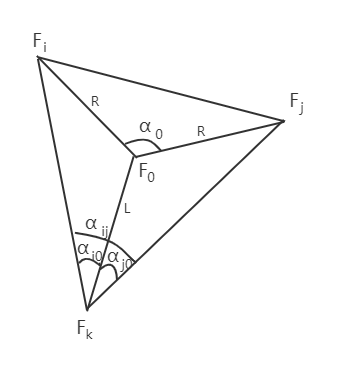
\includegraphics[height=5cm]{./figures/6-1.png}
			\caption{圆形编队接收机情况1}\label{fig:7}
		\end{minipage}
		\begin{minipage}{0.48\linewidth}
			\captionsetup{font={small}}
			\centering
			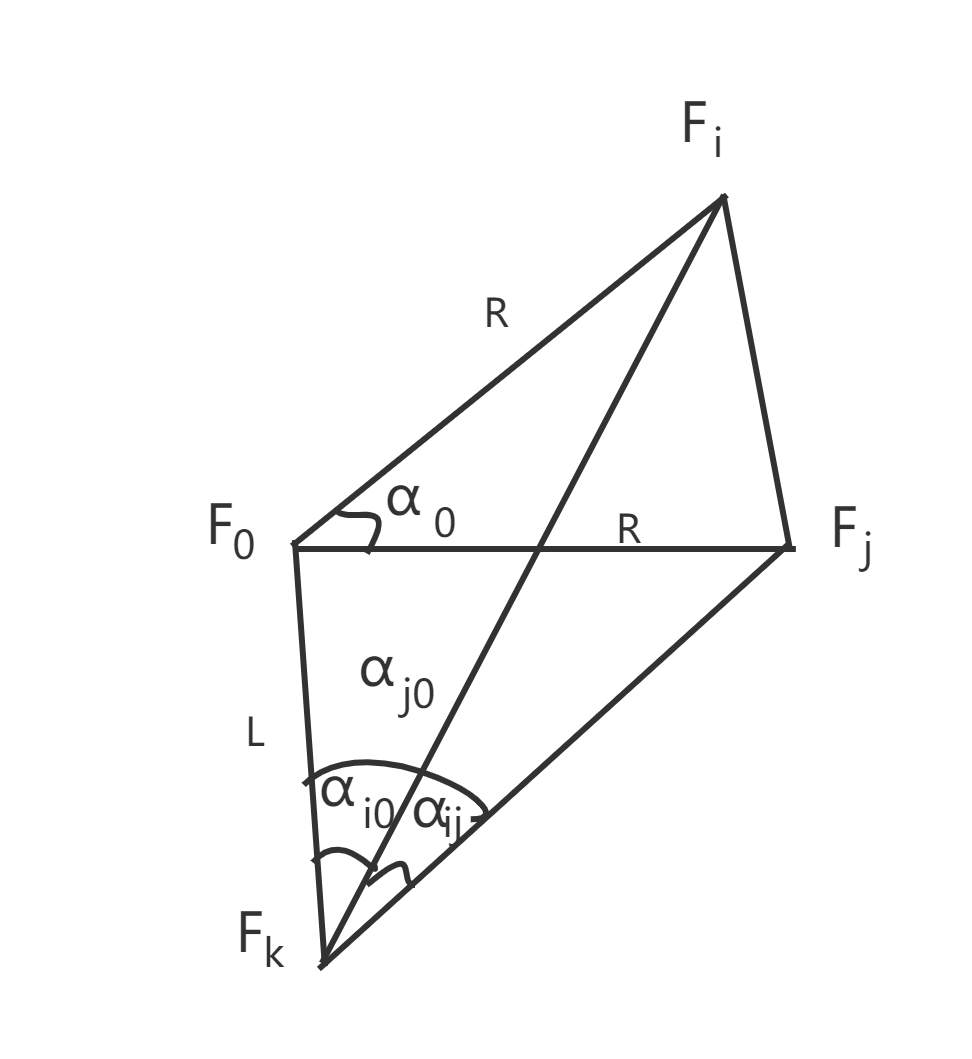
\includegraphics[height=5cm]{./figures/6-2.png}
			\caption{圆形编队接收机情况2}\label{fig:78}
		\end{minipage}
	\end{figure}	
	
	%		由于无人机沿着圆周均匀分布,外围无人机共有九架,假设
	
	令$L=\mid F_{0}F_{k}\mid$,$\angle \alpha_{0} = \angle F_{i}F_{0}F_{j} $,$\angle x = \angle F_{i}F_{0}F_{k}$,在解析题目时,为了便于模型的理解,我们按照圆周上\textbf{两架“发射机”到“接收机”的夹角$\angle \alpha_{ij}$}与\textbf{这两架“发射机”的圆心角$\angle \alpha_{0}$}角度关系组合,进行了多分类讨论,共分出如图4、图5、图6、图7四种几何关系,由\textbf{正弦定理}\cite{zxdl2011}可分别推到出下述四组方程组:
	
	\textbf{情况一\quad}当$90\textdegree<\angle\alpha_{0}<180\textdegree$、$0\textdegree<\angle\alpha_{ij}<90\textdegree$,如图4所示:
	\begin{equation}
		\tag{6-1-2}
		\left\{
		\begin{split}
			\frac{R}{sin\angle \alpha_{i0}} =& 	\frac{L}{sin[180\textdegree-\angle\alpha_{i0}-(360\textdegree -\angle\alpha_{0}-\angle x) ]}
			\\
			=&\frac{L}{-sin[180\textdegree+\angle\alpha_{i0} -\angle\alpha_{0}-\angle x]}\\
			=&\frac{L}{sin[\angle\alpha_{i0} -\angle\alpha_{0}-\angle x]} \\
			\frac{R}{sin\angle \alpha_{j0}} = & 	\frac{L}{sin[180\textdegree-\angle\alpha_{j0}-\angle x]} \\
			= & \frac{L}{sin[\angle\alpha_{j0}+\angle x]}
		\end{split}\right
	\end{equation}
	
	\textbf{情况二\quad} 当$0\textdegree<\angle\alpha_{0}<90\textdegree$、$0\textdegree<\angle\alpha_{ij}<90\textdegree$,如图5所示:
	
	\begin{equation}
		\tag{6-1-3}
		\left\{
		\begin{split}
			\frac{R}{sin\angle \alpha_{i0}} =& 	\frac{L}{sin[180\textdegree-\angle\alpha_{i0}-(\angle\alpha_{0}+\angle x) ]} \\
			\frac{R}{sin\angle \alpha_{j0}} = & 	\frac{L}{sin[180\textdegree-\angle\alpha_{j0}-\angle x]} \\
			= & \frac{L}{sin[\angle\alpha_{j0}+\angle x]}
		\end{split}\right
	\end{equation}
	
	\begin{figure}[!htpb]
		\begin{minipage}{0.48\linewidth}
			\captionsetup{font={small}}
			\centering
			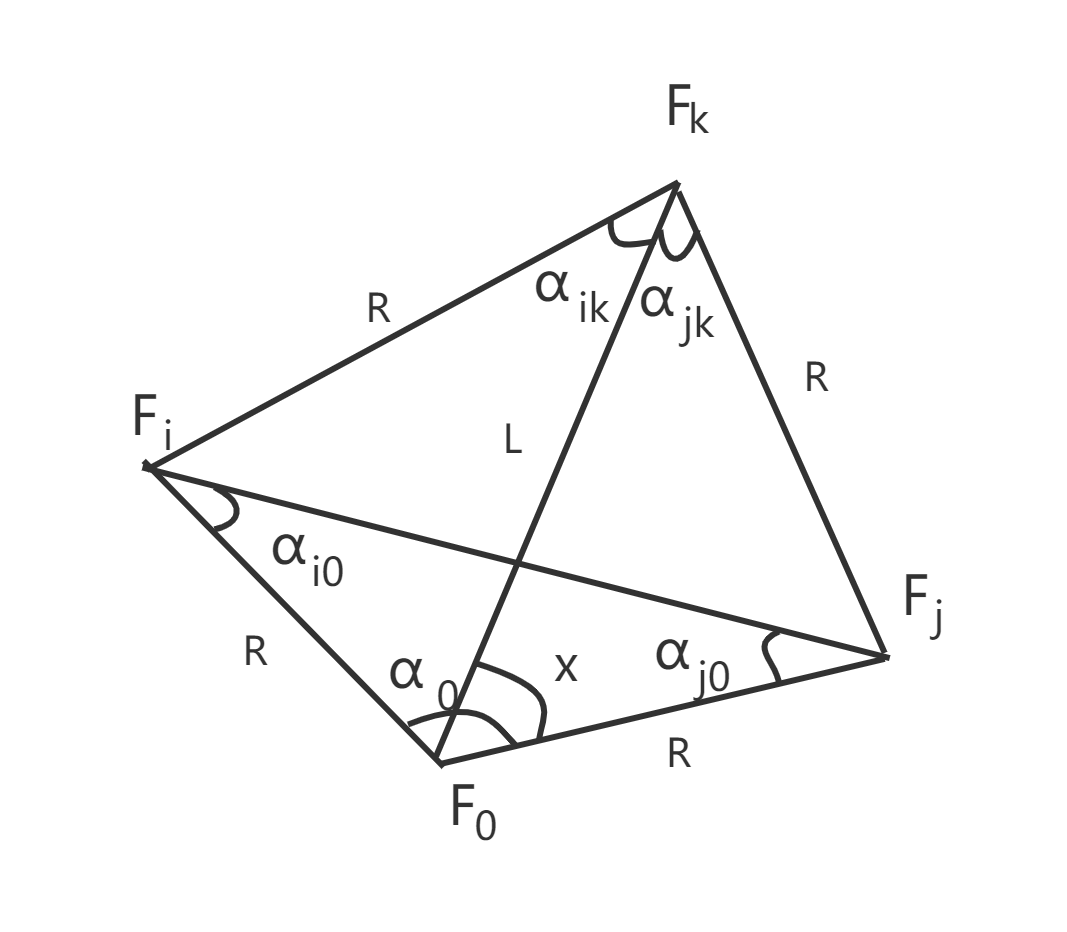
\includegraphics[height=5cm]{./figures/6-3.png}
			\caption{圆形编队接收机情况3}\label{fig:9}
		\end{minipage}
		\begin{minipage}{0.48\linewidth}
			\captionsetup{font={small}}
			\centering
			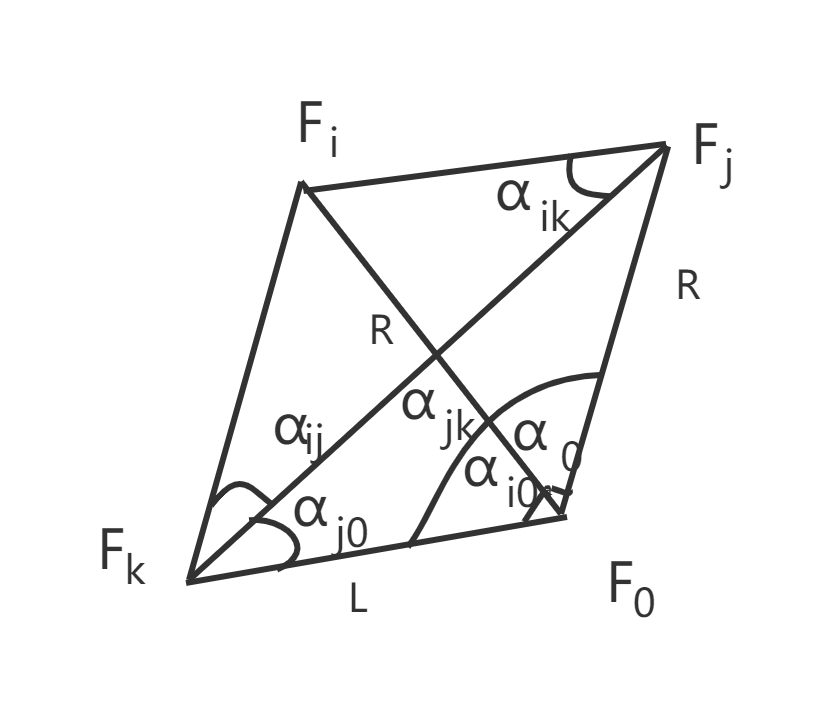
\includegraphics[height=5cm]{./figures/6-4.png}
			\caption{圆形编队接收机情况4}\label{fig:10}
		\end{minipage}
	\end{figure}
	
	\textbf{情况三\quad}	当$90\textdegree<\angle\alpha_{0}<180\textdegree$、$90\textdegree<\angle\alpha_{ij}<180\textdegree$,如图6所示:
	\begin{equation}
		\tag{6-1-4}
		\left\{
		\begin{split}
			\frac{R}{sin\angle \alpha_{ik}} =& 	\frac{L}{sin[180\textdegree-\angle\alpha_{ik}-(\angle\alpha_{0}-\angle x) ]} \\
			\frac{R}{sin\angle \alpha_{jk}} = & 	\frac{L}{sin[180\textdegree-\angle\alpha_{jk}-\angle x]} \\
			= & \frac{L}{sin[\angle\alpha_{jk}+\angle x]}
		\end{split}\right
	\end{equation}
	
	\textbf{情况四\quad}	当$0\textdegree<\angle\alpha_{0}<90\textdegree$、$90\textdegree<\angle\alpha_{ij}<180\textdegree$,如图7所示:
	
	\begin{equation}
		\tag{6-1-5}
		\left\{
		\begin{split}
			\frac{R}{sin[\angle \alpha_{ij}+\angle \alpha_{j0}]} =& 	\frac{L}{sin[180\textdegree-\angle\alpha_{i0}-(\angle \alpha_{ij}+\angle\alpha_{j0})]} \\
			\frac{R}{sin\angle\alpha_{j0}} = & 	\frac{L}{sin[180\textdegree-\angle\alpha_{jk}-\angle j0]} 
		\end{split}\right
	\end{equation}
	
	式6-1-2至6-1-4中均利用\textbf{正弦定理}建立起待求极轴长$L$与各已知夹角$\alpha$之间的关系,在附录B的MATLAB程序中,通过联立方程组消去\textbf{含中间变量$\angle x$}的表达式,便可以解算出待求“接收机”距离圆心的极轴长$L$,solve()为MATLAB内置求解函数,formula表示上述方程组:
	
	\begin{equation}
		\tag{6-1-6}
		[L] = solve(L,formula)
	\end{equation}
	
	%补上最终极角 极坐标
	
	\subsubsection{接收机定位模型精度检验}
	
	在章节6.1.1中,基于纯方位无缘定位法我们对信号“发射机”和“接收机”的相对集合关系进行了数学解析,通过解析法设计了可以计算极轴长$L$的几何模型,从而定位出了“接收机”的极坐标。为了进一步验证模型的可靠性,我们使用章节5.1中制作的模拟集对
	6.1.1的模型进行检验,最终得出\textbf{置信水平高达0.999}。
	
	\begin{figure}[htbp!]
		\captionsetup{font={small}}
		\centering
		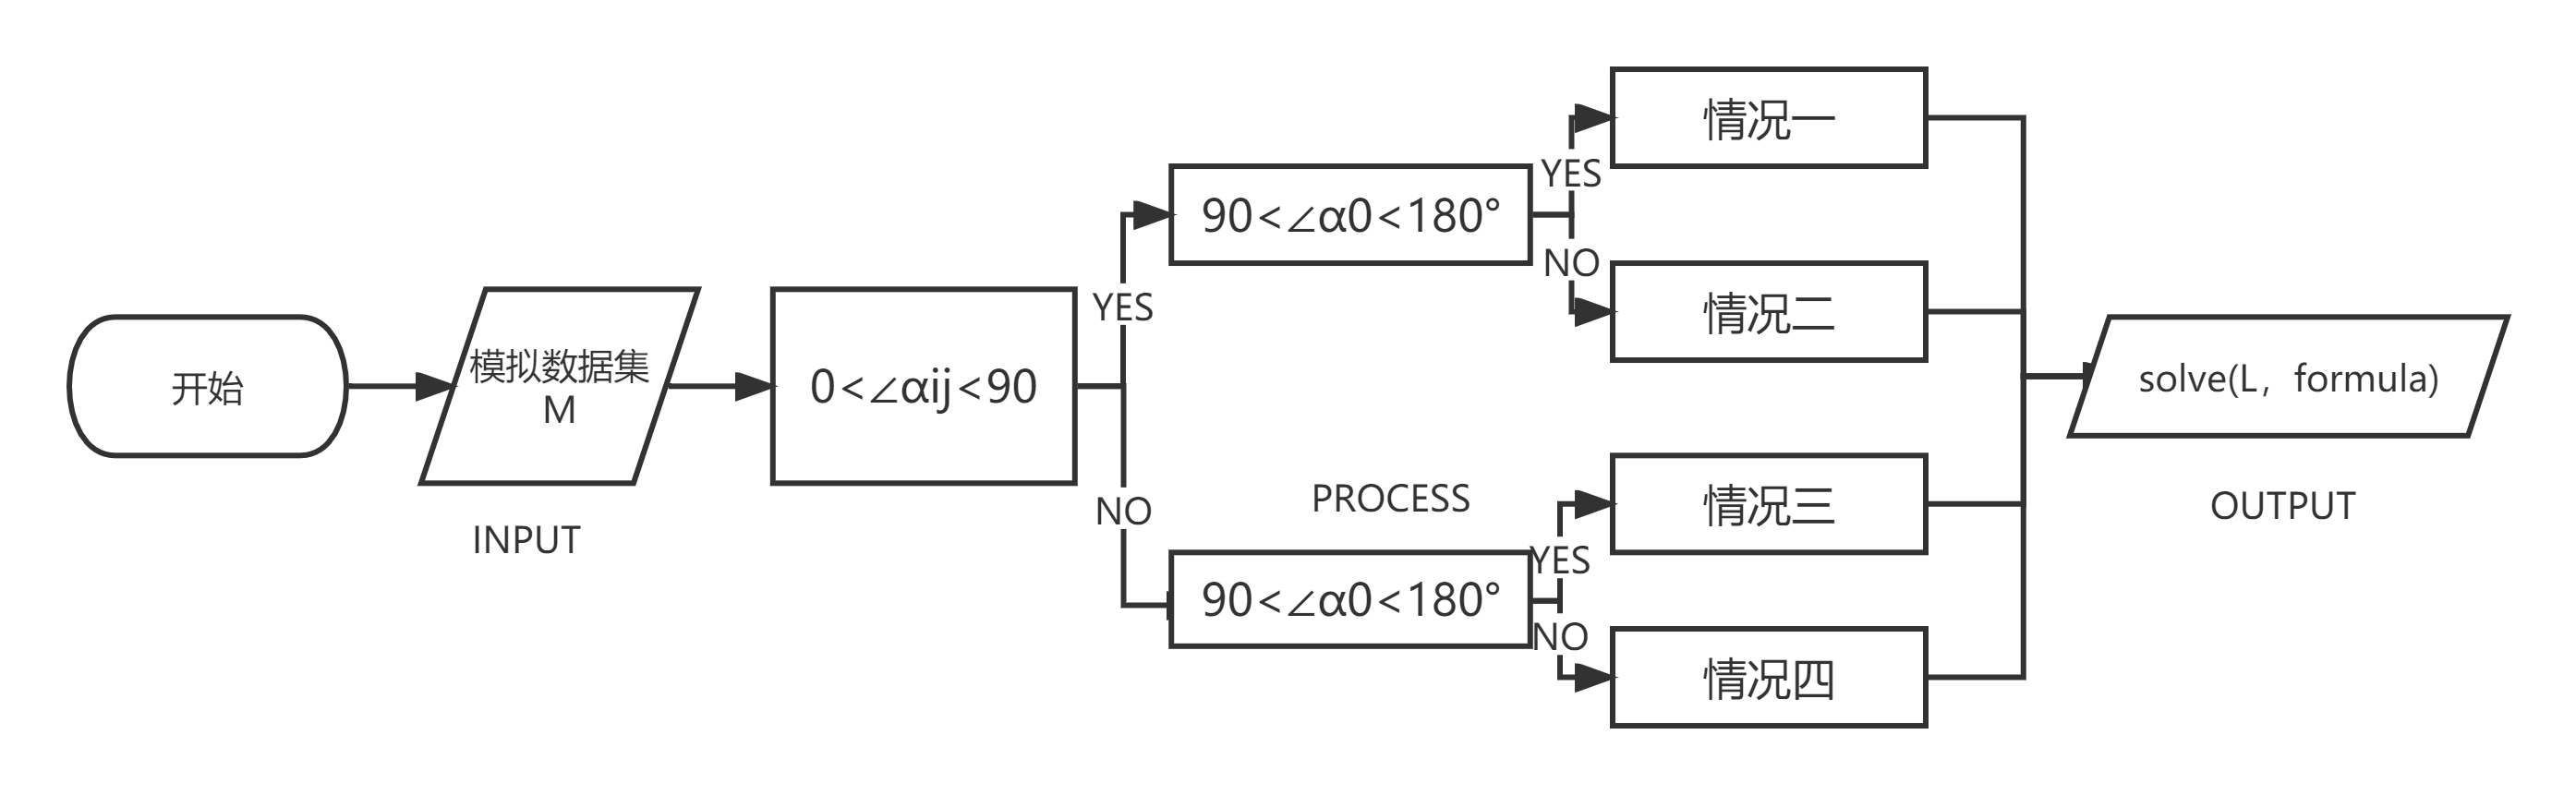
\includegraphics[height=4.5cm]{./figures/6-6.png}
		\caption{情况讨论分支语句流程图}\label{fig:10}
	\end{figure}
	\newpage
	\noindent\textbf{Step.1}
	
	将模拟集中的元素遍历,依次将$F_{i}$、$F_{j}$、$F_{k}$模拟数据中的$\alpha_{ij}$、$\alpha_{0}$进行比较,在MATLAB程序中使用分支语句进行分类,依次归入四种情况。
	
	\noindent\textbf{Step.2}
	
	将模拟集中的元素遍历,依次将$F_{i}$、$F_{j}$、$F_{k}$模拟数据带入四种情况的求解模型中,依次计算出7架“接收机”的极角$\theta_{k}'$、极轴长$\rho_{k}'$。
	
	\noindent\textbf{Step.3}
	
	通过依次比较原始数据和求解数据,若同时满足:
	\begin{equation}
		\tag{6-1-7}
		\left\{
		\begin{split}
			\rho_{k} =\rho_{k}'\\
			\theta_{k} =\theta_{k}'
		\end{split}\right
	\end{equation}
	
	则认为对模拟数据中“接收机”方位的定位正确,计数$count++$自增1个单位,最终使用成功试验次数与总试验次数的频率来描述模型定位程度的置信水平$Z$,最终求得$Z\approx0.999$,如表2所示,取前10条模拟数据,表中10组数据均准确的定位到模拟出的无人机的极坐标,当观测接收机相对方位角$\alpha_{1}=28.8594$、$\alpha_{2}=66.2404$、$\alpha_{3}=95.0998$时,预测出观测点坐标为(105.2242,239.3820\textdegree)为完整数据详见附录F:
	
	\begin{equation}
		\tag{6-1-8}
		Z= \frac{count}{101} 
	\end{equation}
	
	\begin{table}[htbp!]
		\small
		\captionsetup{font={small}}
		\caption{“接收机”定位模型验证数据表(前10条)}
		\centering
		%					\renewcommand\arraystretch{4}
		\tabcolsep=0.1cm
		\begin{tabular}{@{}ccccccccc@{}}
			\toprule
			\textbf{接收机编号} & \textbf{发射机编号} & \textbf{$\alpha_{i}$} & \textbf{$\alpha_{j}$} & \textbf{$\alpha_{0}$} & \textbf{真实位置极径} & \textbf{真实位置极角} & \textbf{模型输出极径} & \textbf{模型输出极角} \\ \midrule
			6              & 7              & 28.8594     & 66.2404     & 95.0998     & 105.2242        & 239.3820        & 105.2242        & 239.3820        \\
			2              & 3              & 50.9066     & 72.2338     & 21.3272     & 97.0403         & 80.2295         & 97.0403         & 80.2295         \\
			4              & 6              & 10.1527     & 47.9040     & 58.0567     & 105.1239        & 200.8316        & 105.1239        & 200.8316        \\
			9              & 3              & 48.8287     & 29.3571     & 19.4715     & 103.0628        & 80.2937         & 103.0628        & 80.2937         \\
			6              & 8              & 50.0504     & 49.6488     & 99.6993     & 100.4413        & 280.4038        & 100.4413        & 280.4038        \\
			2              & 3              & 47.2977     & 63.4888     & 16.1911     & 108.8599        & 79.5724         & 108.8599        & 79.5724         \\
			6              & 2              & 72.1601     & 9.7031      & 81.8632     & 97.8389         & 39.1946         & 97.8389         & 39.1946         \\
			5              & 7              & 29.7529     & 49.3822     & 79.1351     & 101.7220        & 240.0714        & 101.7220        & 240.0714        \\
			8              & 2              & 69.5583     & 29.8101     & 39.7482     & 100.4087        & 40.2456         & 100.4087        & 40.2456         \\
			5              & 8              & 51.3596     & 30.7755     & 82.1350     & 95.8703         & 279.8482        & 95.8703         & 279.8482        \\ \bottomrule
		\end{tabular}
	\end{table}
	
	\subsection{未知发射机编号时使发射机数量最少}
	
	在章节6.1.2中,通过计算机模拟,使用101组试验数据验证了(1)小问中的模型精度,且(1)题背景下只使用了3架发射机,数量较少。据此,我们认为该模型的有较高精度同时可以发射较少的电磁波,在(2)小问中仍可运用该模型推算“发射机”的配置:
	
	\subsubsection{衡量无人机编队定位准确度的损失函数}
	
	为了同时描述无人机编队的定位精度和机队的数量,在章节5.2中通过计算机模拟,生成了100组测试数据。而由6.1.2中的试验可知,当(2)小问中“发射机”选取越接近采样点的情况时,回带6.1.1的“接收机”定位模型准确度越高。
	
	据此,我们定义“发射机”选取会影响“接收机”定位精度,且可用一损失函数$Loss$对影响进行评价。选取一架的外围无人机与FA00、FA01号共同作为“发射机”,模拟原始数据为“第k架无人机的原始极坐标为$(\rho_{k},\theta_{k})$”,对应第k架无人机的测试极坐标为$(\rho'_{k},\theta'_{k})$:
	
	\begin{equation}
		\tag{6-2-1}
		Loss_{k} = \sqrt{\rho_{k}^{2}+\rho_{k}'^{2}-2\rho_{k}\rho_{k}'cos(\theta_{k}-\theta_{k}')}
	\end{equation}
	
	\subsubsection{全局搜索获取新增一架“发射机”的编号}
	
	在(1)小问模型基础上,以40\textdegree 设置旋转梯度,假设外围无人机恰好以逆时针递增次增编号,分别为01$\sim$09。以FA00与FA01连线的正方向作为无人机编队极坐标体系的初始位置。依次将$F_{k}$作为新增的一架“发射机”,$F_{k}$的极坐标可以表示为(R,$\frac{(k-1)\pi}{9}$)
	
	在章节5.2中我们模拟出了100组符合条件的数据,可以将数据集“N”作为原始集。对除了FA00和FA01号外的其他无人机进行一次全局遍历搜索,每次选取FA0i($F_{i}$)号无人机作为新增“发射机”。
	
	每轮修改“发射机”编号后,都要依次对所有计算式6-2-1所示的损失函数值$Loss_{k}$。在遍历过程中使用如式6-2-2所示的\textbf{“优化函数”}对“发射机”的选取进行评估。
	
	\begin{equation}
		\tag{6-2-2}
		min\quad min[Loss]  
	\end{equation}
	
	当损失值趋于0时,说明无人机的原始数据与圆周上的标的点非常接近。
	
	\subsubsection{只取一架“发射机”无法完全实现精确定位}
	
	基于上文的分析,我们使用损失函数$Loss$做了全局搜索。对于部分样本点,3架“发射机”可以得出检测无人机的序号;但是,存在部分样本点出现了异常值,再重复试验发现该组点存在多个结果。
	
	结合图9,经过考虑和研讨,我们认为多解问题主要是由于“发射机”的选取可能有等价情况。
	由于外围共有9架均匀分布的无人机,沿着FA00与FA01延长线呈轴对称。对于同一组定位目标,可能存在两组对称的最优“发射机”选择方案,如图所示,故仅用3架“发射机”无法实现定位的完全精确:
	
	%					\begin{figure}[htbp!]
	%						\captionsetup{font={small}}
	%						\centering
	%						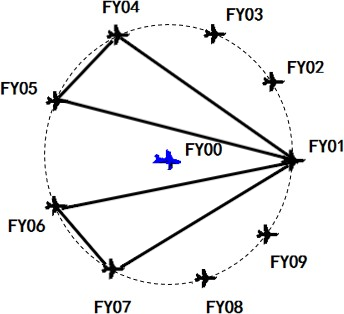
\includegraphics[height=5cm]{./figures/6-7.png}
	%						\caption{同一接收机定位有对称的发射机选取方案}\label{fig:11}
	%					\end{figure}
	
	\begin{figure}[!htpb]
		\begin{minipage}{0.48\linewidth}
			\captionsetup{font={small}}
			\centering
			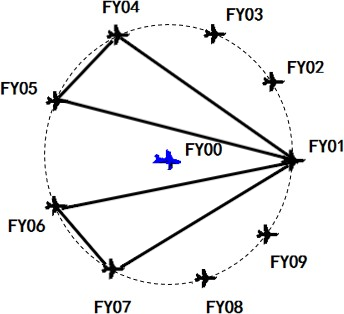
\includegraphics[height=5cm]{./figures/6-7.png}
			\caption{同一接收机定位等价发射机选取方案(实例一)}\label{fig:19}
		\end{minipage}
		\begin{minipage}{0.48\linewidth}
			\captionsetup{font={small}}
			\centering
			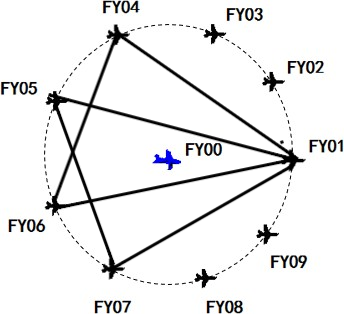
\includegraphics[height=5cm]{./figures/6-8.png}
			\caption{同一接收机定位等价发射机选取方案(实例二)}\label{fig:20}
		\end{minipage}
	\end{figure}
	
	\subsubsection{全局搜索获取新增两架“发射机”的编号}
	
	在章节6.2.1中我们只选了一架“发射机”但发现存在对称多解,故需要继续增加“发射机”的数量。故,我们考虑获取新增2架“发射机”的编号。
	
	同时,由于“发射机”数量的改变提高了定位的精度,损失函数的实际意义失效;需要随之调整,如式6-2-3所示,选用FA00、FA01和另选中两架$F_{i}$、$F_{j}$作为“发射机”,可以分别取FA00、FA01、$F_{i}$作为第一组定位信号“发射机”,按照式6-2-1计算出损失函数值$Loss^{(1)}$;同理再取FA00、FA01、$F_{j}$作为第二组“发射机”,计算损失函数值趋于最小,达到最优:
	\begin{equation}
		\tag{6-2-3}
		min \quad min[Loss^{(1)}_{k} + Loss^{(2)}_{k}]  
	\end{equation}
	
	从除了FA00和FA01号外的其他无人机进行嵌套遍历,每组挑选出两架新增“发射机,记为“FA0i($F_{i}$)、FA0j($F_{j}$)”。对所选的数据组,以横轴为第一组的函数损失值,纵轴为第二组的损失值,绘制如图10所示的损失函数值图像。从图中不难发现,大部分点落在半径为100m的圆内,即大部分区域可以被准确定位出。
	
	\begin{figure}[htbp!]
		\captionsetup{font={small}}
		\centering
		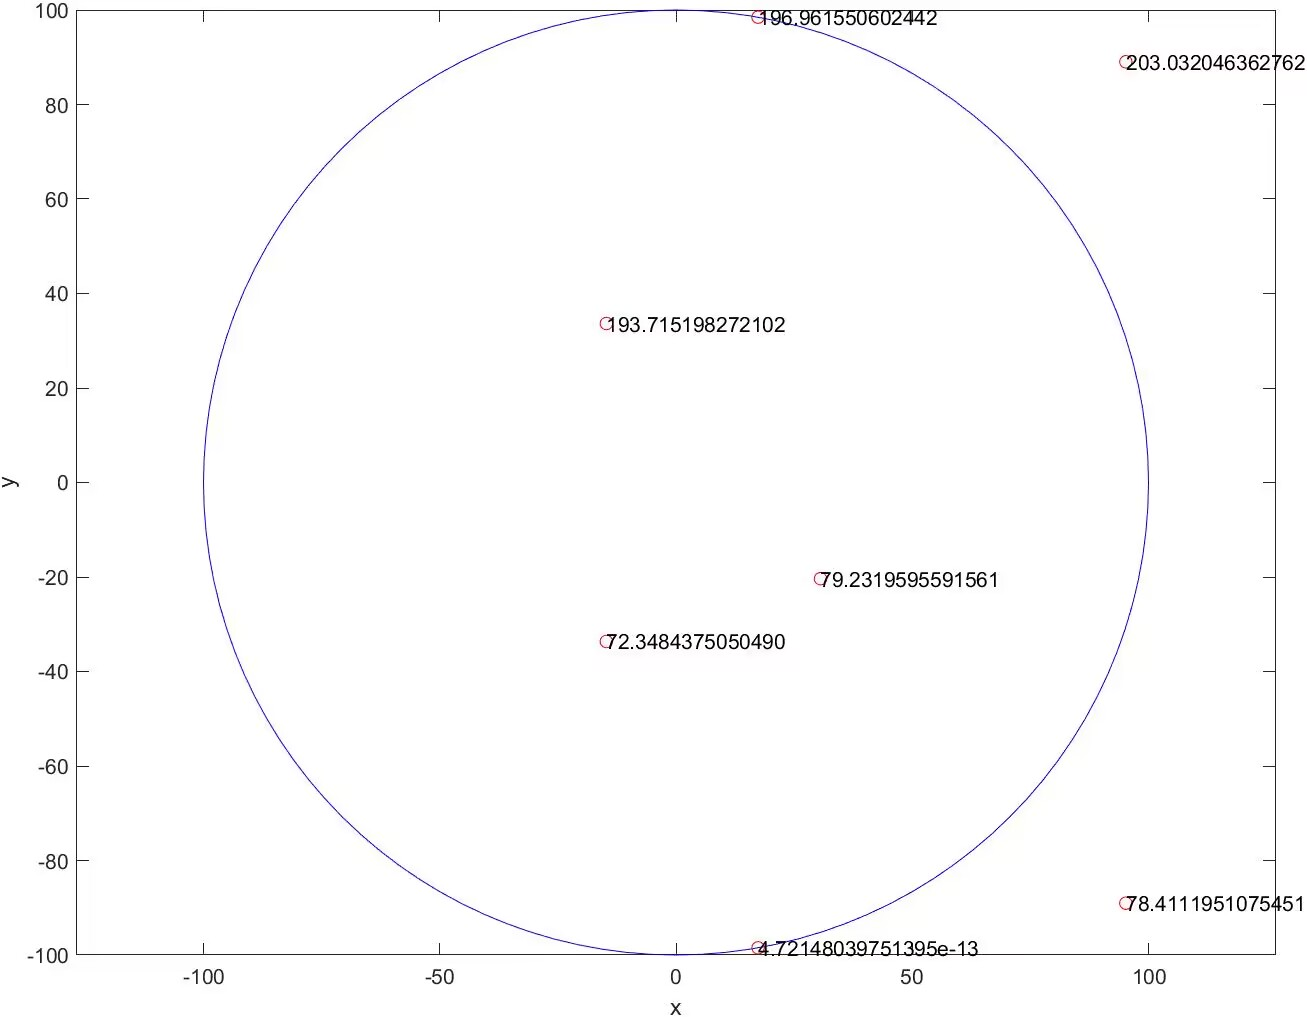
\includegraphics[height=6cm]{./figures/6-9.jpg}
		\caption{选取新增两架“发射机”时测试集的损失值雷达图}\label{fig:13}
	\end{figure}
	
	\subsubsection{第(2)小问结论}
	
	(1)测试检验:
	
	为了检验本模型对另外增选“发射机”模型的准确度,我们仿照(1)小问中计算机模拟的思路,根据章节5.2中模拟出的测试集数据,通过带回模型的方式,统计通过无人机序号检验的实验次数,最终得出本模型可以完美地准确解析出“发射机”的序号。拥有4架“发射机”后,基于章节6.1中定位模型的研究,最终可计算出所有无人机的方位信息。如表3所示,列举了前10条模拟检验数据,可依照“相对方位角$\alpha$”检验模型精度。如表3所示,当选取两架无人机发射角分别为:新增第一架“发射机”中$\alpha_{1}$为9.7917,	$\alpha_{2}$为52.1907,$\alpha_{1}$为61.9825,第二架“发射机”中$\alpha_{1}$为9.7917,	$\alpha_{2}$为31.2953,$\alpha_{1}$为40.0871时,可以准确的分辨出FYX1号无人机为 “FY07号”、FYX1号无人机为 “FY08号”等,可以反映出模型具有优秀的测试效果,完整数据详见附录F。
	
	% Please add the following required packages to your document preamble:
	% \usepackage{booktabs}
	\begin{table}[htbp!]
		\footnotesize
		\captionsetup{font={small}}
		\caption{无人机序号识别检验数据表(前10条)}
		\centering
		%					\renewcommand\arraystretch{4}
		\tabcolsep=0.1cm
		\begin{tabular}{@{}cccccccccc@{}}
			\toprule
			\multicolumn{3}{c}{\textbf{FYX1发射机对应的发射角}}                                                           & \multicolumn{3}{c}{\textbf{FYX2发射机对应的发射角}}                                                           & \textbf{FYX1的真实编号} & \textbf{FYX2的真实编号} & \textbf{FYX1模型识别编号} & \textbf{FYX2模型识别编号} \\ \midrule
			\multicolumn{1}{c|}{\textbf{$\alpha_{1}$}} & \multicolumn{1}{c|}{\textbf{$\alpha_{2}$}} & \multicolumn{1}{c|}{\textbf{$\alpha_{3}$}} & \multicolumn{1}{c|}{\textbf{$\alpha_{1}$}} & \multicolumn{1}{c|}{\textbf{$\alpha_{2}$}} & \multicolumn{1}{c|}{\textbf{$\alpha_{3}$}} & \multicolumn{4}{c}{\textbf{}}                                                                 \\ \midrule
			9.7917                           & 52.1907                          & 61.9825                          & 9.7917                           & 31.2953                          & 41.0871                          & 7                    & 8                    & 7                      & 8                      \\
			66.6277                          & 29.8035                          & 96.4311                          & 66.6277                          & 9.3708                           & 57.2568                          & 5                    & 7                    & 5                      & 7                      \\
			46.5893                          & 62.7189                          & 16.1296                          & 46.5893                          & 28.8778                          & 75.4670                          & 2                    & 6                    & 2                      & 6                      \\
			30.8234                          & 75.4210                          & 44.5976                          & 30.8234                          & 10.8140                          & 41.6374                          & 3                    & 8                    & 3                      & 8                      \\
			65.1491                          & 64.9471                          & 130.0962                         & 65.1491                          & 9.8149                           & 55.3343                          & 3                    & 7                    & 3                      & 7                      \\
			64.9607                          & 28.6424                          & 36.3183                          & 64.9607                          & 47.5875                          & 17.3732                          & 8                    & 9                    & 8                      & 9                      \\
			65.1266                          & 48.1506                          & 16.9760                          & 65.1266                          & 29.3292                          & 35.7974                          & 2                    & 3                    & 2                      & 3                      \\
			30.8349                          & 30.7603                          & 61.5951                          & 30.8349                          & 51.6842                          & 20.8493                          & 4                    & 9                    & 4                      & 9                      \\
			53.1828                          & 78.4849                          & 131.6677                         & 53.1828                          & 10.8320                          & 64.0148                          & 4                    & 7                    & 4                      & 7                      \\
			48.2132                          & 10.1367                          & 38.0765                          & 48.2132                          & 47.3229                          & 95.5361                          & 3                    & 6                    & 3                      & 6                      \\ \bottomrule
		\end{tabular}
	\end{table}
	(2)结论小结:
	
	本题中,为了实现有效的无人机定位,同时尽可能减少电磁波的干扰,保持定位的准确性和可靠性;除FY00和FY01外,还至少需要\textbf{再选2架}“发射机”。
	
	\subsection{择优选取信号发射机以动态调整无人机编队位置}
	
	\subsubsection{动态调整“发射机”排布位置}
	
	本题中“发射机”的选取会随着机队调整而改变,为了实现最终无人机编队整体整齐,可能会进行多次变换调整。无人机编队是一个集群系统,系统中的成员异动会引发其他成员的姿态调整反应。同时,根据题目约束条件,“发射机”可能存在位置偏差。不妨从编队以FA00号机为参考系的角度思考,则外围9架无人机均需要各自向着坐标已知的位置移动。
	
	查阅资料,无人机的位置运动,需要同时在位移指令中告知该无人机的\textbf{初始坐标}和\textbf{目标坐标}
	在表1中给出的数据中,FA00与FA01号无人机已分别精准地布于目标位置(0,0)和(100,0),根据章节6.1中的“接收机”定位模型,只要再有一架“发射机”达到给定目标位置后,便可以99.9\%的置信水平下精准卡尔曼滤波器是一种适用于线性系统中未知环境下理想参数估计的数据最优化自回归处理方法,对存在误差的观测值也能够有效地估计真实值。本题中,无人机中由“发射机”引导“接收机”调整位置,而定位出其他“接收机”的坐标。根据这组精确坐标与运动目标坐标,可以计算出\textbf{飞行方向}和\textbf{步长}。我们考虑在章节6.1的定位模型和6.2“发射机”选择模型的基础上再做改进。
	
	%					画图
	承上述分析,无人机的\textbf{初始坐标}和最终希望达到的\textbf{目标坐标}已知。首先,需要让2-9号无人机中其中一架在目标位置到位。参考6.2的“发射机”选择模型,需要在移动的过程中准确地告知“接收机”的实时坐标,由于该机初始位置的轴长扰动$\epsilon$,初始时找不到三架无偏差的“发射机”,只能用其中坐标最接近于目标的一架取代;由此,该定位体系此时得出的\textbf{其他无人机的定位坐标}是不精确的,据此的位移指令也是不精确的。故本题需使用一种可以\textbf{应对带“扰动”数据}的处理方法,\textbf{卡尔曼滤波器}算法符合本题的实际需求。
	
	
	\subsubsection{卡尔曼滤波器}
	
	(1)卡尔曼滤波器简介:
	
	传统的卡尔曼滤波器是一种适用于线性系统中未知环境下理想参数估计的数据最优化自回归处理方法,对存在误差的观测值也能够有效地估计真实值。本题中,无人机中由“发射机”引导“接收机”调整位置,而“发射机”的位置围绕着圆周轨迹具有一定的扰动$\epsilon$,自身的牵引信号存在一定偏差,而卡尔曼滤波器可以折中地处理由观测源数据误差引起的整体失调,(3)小问选用卡尔曼滤波器主要是由此考虑。算法中卡尔曼滤波算法基本实现原理主要包含预测和更新两部,分别对应无人机位置调整循环周期内的两个阶段:
	
	(2)预测:
	
	由于卡尔曼滤波算法评估的对象的状态向量是动态调整,为了避免“后馈”响应模式下导致的滞后局限性,在调整状态之前需通过“预测状态向量”实时跟进评估状态变化态势。
	
	
	(3)更新:
	
	编队中任意无人机位置的调整,若仍然保持上一次响应设定的状态参数,会引起机队整体的偏移。故每当“发射机”施加调整指令之后,都需要及时响应,将新状态下应保持的编队极坐标参数更新到对应的机位上。
	
	\subsubsection{自适应的卡尔曼滤波算法}
	
	\begin{figure}[htbp!]
		\captionsetup{font={small}}
		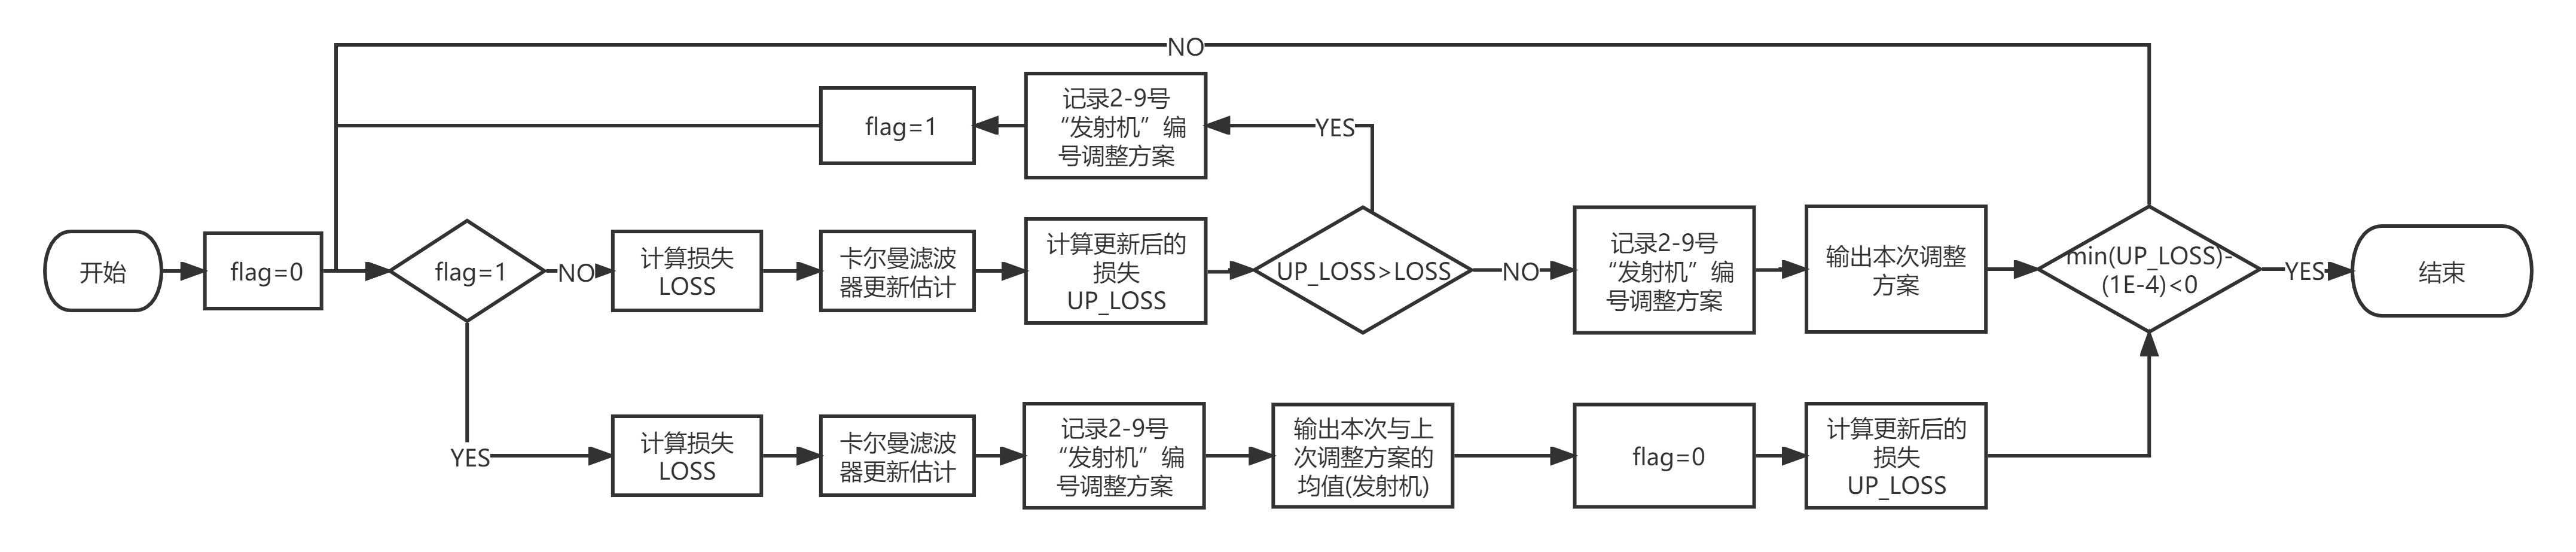
\includegraphics[width=16.5cm]{./figures/6-10.png}
		\caption{自适应卡尔曼滤波器架构图}\label{fig:12}
	\end{figure}
	
	在卡尔曼滤波器中,通常以先验估计对短期内的机队形态变化做预测,通过后验概率对结论进行检验,经过反复的参数调整,最终编队整体形态达到目标。
	
	(1)无人机的状态向量:
	
	本题中,在章节6.1的“接收机”定位模型中,无人机的方位信息为无人机所处的极坐标($\rho$,$\theta$);同时初始状态各无人机的极坐标已给出,不用再进行初始化。
	\begin{equation}
		\tag{6-3-1}
		\vec{X_{k}} = \begin{bmatrix}
			\rho_{k}\\
			\theta_{k}
		\end{bmatrix}
	\end{equation}	
	
	对于二维的状态向量,要想解析出无人机的实时状态、预测未来状态并据此给出相应的机队调整方案:
	
	(2)协方差函数:
	
	\begin{equation}
		\tag{6-3-2}
		\begin{split}
			U_{i} & = \frac{\sum_{k=1}^{n} X_{k}}{n} \\
			\sum_{ij} & = Cov(X_{i},X_{j}) = E[(X_{i}-U_{i})(X_{j}-U_{j})]
		\end{split}
	\end{equation}
	
	(3)协方差矩阵:
	
	\begin{equation}
		\tag{6-3-3}
		P_{k} =	\begin{bmatrix}
			\sum_{\rho\rho} &\sum_{\rho\theta} \\
			\sum_{\rho\theta} & \sum_{\theta\theta}
		\end{bmatrix}
	\end{equation}
	
	为了描述调整编队形态的过程的不确定性, 按卡尔曼滤波算法,需要从状态向量的协方差入手分析,依据协方差的定义,可以计算出第i次调整与第j次调整间的协方差$\sum_{ij}$如式6-3-2;为便于推演,将算得协方差以式6-3-3所示的协方差矩阵形式表示为$P_{k}$。之后,根据协方差的乘法运算,可以把协方差阵变形为式6-3-4的形式,其中Cov()为求协方差函数:
	
	\begin{equation}
		\tag{6-3-4}
		Cov(AX) = A\sum A^{T}
	\end{equation}
	
	(4)先验状态估计:
	
	无人机编队飞行以当前极坐标($\rho$,$\theta$)来表征无人机所处状态,故本题中使用无人机极坐标来作为先验状态向量。
	
	先验概率估计是一种假设检验方法,先验估计$\hat{X_{k}}$主要取决于三个方面:
	
	\qquad	(a)无人机编队前一次调整的最优估计;
	
	\qquad (b)环境当中存在一定的噪声干扰;
	
	\qquad (c)确定的外部影响值。
	
	为了描述跟踪对象的变化,需要通过先验估计计算状态向量的协方差矩阵$P_{k}$,预测出可能的调整趋势。
	
	由于环境中存在无法线性描述的误差(“发射机”不一定在圆周上),需要在预测时允许有一定扰动,用$R_{k}$表示环境不确定度,且状态变化过程受外界的影响,用$O_{k}$表示,则有状态预测公式,如式6-3-5:
	\begin{equation}
		\tag{6-3-5}
		\begin{split}
			\hat{X}_{k} &=Q_{k} \hat{X}_{k-1} + S{k}O_{k}\\
			P_{k} &=Q_{k} P_{k-1}Q_{k}^{T} + R_{k}
		\end{split}
	\end{equation}	
	其中$Q_{k}$为状态变量的转移矩阵,由于在题目中经过假设:\textbf{无人机位置调整认为"瞬间"完成},状态变化转换为非线性,无法直接解析出$Q_{k}$的变化过程;同理,$S_{k}$为状态参数异动,故本处不对$Q_{k}$、$S_{k}$注解。
	
	(5)后验检验:
	
	为了校验无人机编队位置调整的合理性,每次无人机的矫正都需要进行一次损失函数评估。与章节6.2.1中对损失函数的定义类似,本题中讨论损失的对象是除了FA00、FA01号无人机以外的其它成员,对2$\sim$9号无人机我们建立列表,每轮调整都记录下$F_{2} \sim F_{9}$对应的每组损失值$Loss_{k}$,以总体损失值来检验无人机编队调整的优度:
	%    						Loss_{k} &= \sqrt{\rho_{k}^{2}+\rho_{k}'^{2}-2\rho_{k}\rho_{k}'cos(\theta_{k}-\theta_{k}')}\\
	\begin{equation}
		\tag{6-3-6}
		\begin{split}
			Loss_{k} & = \frac{(\rho_{k}' - \rho_{k})^{2}}{\sum_{k=2}^{9}(\rho_{k}' - \rho_{k})^{2}} + \frac{(\theta_{k}' - \theta_{k})^{2}}{\sum_{k=2}^{9}(\theta_{k}' - \theta_{k})^{2}}  \\
			&min\quad\sum_{k=2}^{9}Loss_{k}
		\end{split}
	\end{equation}	
	
	当损失函数值合趋于最小时,说明观测值和预测值十分接近,可以认为“先验估计是可靠的”,该调整方案已可达到预测的最优状态。
	
	(4)卡尔曼滤波参数更新:
	
	每一轮无人机编队的调整后,都需要对编队的状态向量更新,类似于动态优化模型,如下式,$U_{i}$为输入向量中第i次变换后的状态向量均值,$\sum$为状态变量的协方差,$U'$表示当前更新后的均值,$H_{k_{i}}$为第i个有预测值到观测值的变换矩阵,$\sum$'表示当前更新后的协方差:
	\begin{equation}
		\tag{6-3-7}
		\begin{split}
			k'_{i}&= \sum_{i}( \sum_{i}+ \sum_{i+1})^{-1}\\
			&= \frac{H_{k'_{i}}P_{k'_{i}}H_{k'_{i}}^{T}}{H_{k'_{i}}P_{k'_{i}}H_{k'_{i}}^{T}+R_{k'_{i}}} \\
			U'&= U_{i}+ k'(U_{i+1}- U_{i}) \\
			\sum'& = \sum_{i} - k'_{i}\sum_{i} \\
			P'_{k'}& =P_{k}-k'H_{k'_{i}}P_{k}
		\end{split}
	\end{equation}
	
	
	
	(6)算法程序实现步骤:
	
	\noindent\textbf{Step.1}
	
	根据表1中给出的无人机坐标进行首次调整,需要再选一架合适“发射机”。我们依据式6-3-6,计算了损失函数值$Loss$(MSE),选取损失值最小的作为第一轮调整的新增“发射机”。
	
	\noindent	\textbf{Step.2}
	
	以选中的3架“发射机”为参考,依据上文中(1)(2)(3)(4)(5)小结算法阐述,对其余的“接收机”进行反复多轮\textbf{“卡尔曼滤波”}。据此可以得出对全体无人机的\textbf{坐标估计值}。
	
	\noindent	\textbf{Step.3}
	
	当\textbf{坐标估计值}在误差范围内,,基于6.3.3中对卡尔曼滤波的论述,当式6-3-6中的损失函数值$Loss_{k}$趋于最小且在扰动$\epsilon <1E-4$时,可认为此时该机的坐标的准确的,便可命令让该机运动到目标位置。
	
	\noindent	\textbf{Step.4}	
	
	当所有无人机都运动到目标位置后,此时的无人机编队实现了在圆形形态的稳定。
	
	根据章节6.1中的“接收机”定位模型、3架位置无偏差“发射机”的方位信息$F_{i}$、$F_{j}$、$F_{0}$和其他无人机的相对方位角$\alpha$,便可以依次计算出“接收机”的坐标($\rho_{k}$,$\theta_{k}$);最后,对比当前“接收机”的坐标和已知的目标坐标,便可以计算出运动方向$\theta$和步长$\rho_{b}$:
	
	\begin{equation}
		\tag{6-3-8}
		\left\{
		\begin{split}
			\theta_{2} &=\pi+\theta_{3} \\
			\rho_{b} &=\rho_{a}\cdot\frac{sin\theta_{3}}{sin\theta_{1}} 
		\end{split}\right
	\end{equation}
	
	\begin{figure}[htbp!]
		\centering
		\captionsetup{font={small}}
		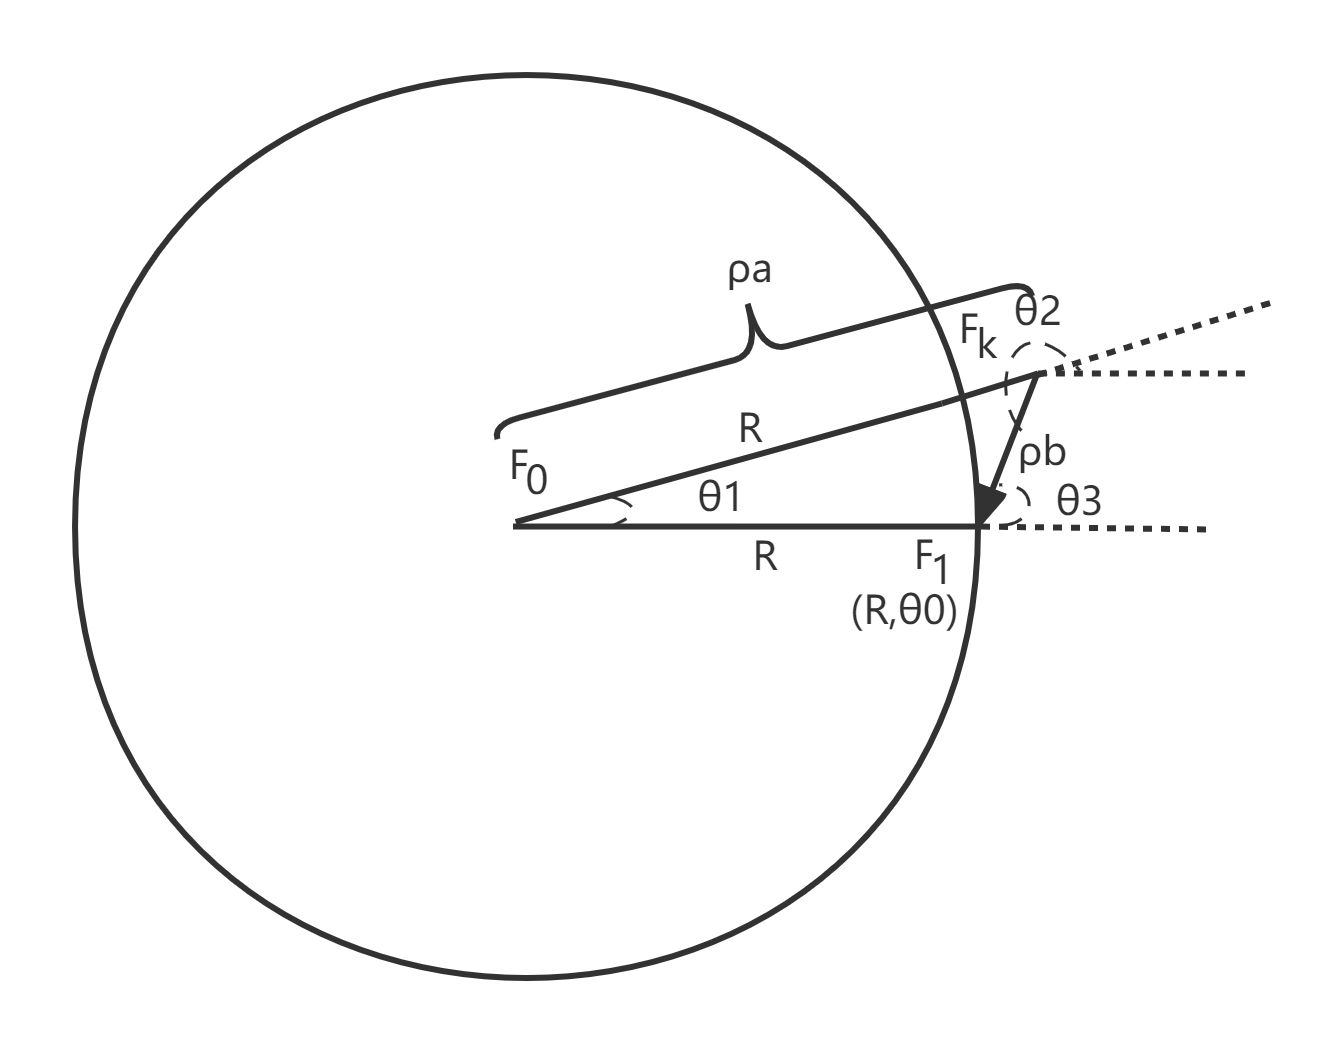
\includegraphics[height=4.5cm]{./figures/6-12.png}
		\caption{运动方向、步长示意图}\label{fig:14}
	\end{figure}
	\subsubsection{第(3)小问结论:编队调整方案}	
	
	\section{问题二模型}	
	
	\subsection{考虑无人机编队型态变换}
	
	问题二中无人机编队调整与问题一(3)小问中的情况类似,本题将继承该问的条件约束。由于编队队形改变为锥形,需要重新考虑建系、信号“发射机”等选取。先就队形调整引起的条件变化重新约定:
	
	\subsubsection{锥形编队下坐标系的建立}
	
	为了使章节6.3中的无人机编队矫正模型适用,保证问题的线性特性;本题中仍然考虑使用极坐标体系:
	
	(1)极心的约定:
	
	在锥形编队下,无人机集群一共有15架按正三角形分布,即任意相邻两架无人机间的距离都相等,不妨记间距为$R$(以$R=50m$为例)。同时为了便于程序设计和模型表达,应尽量时更多的坐标点落在周上。经过试验,我们最终选取以FA13号无人机作为机队集群的极心,逆时针方向为正方向,如图13所示:
	-		
	\begin{figure}[htbp!]
		\centering
		\captionsetup{font={small}}
		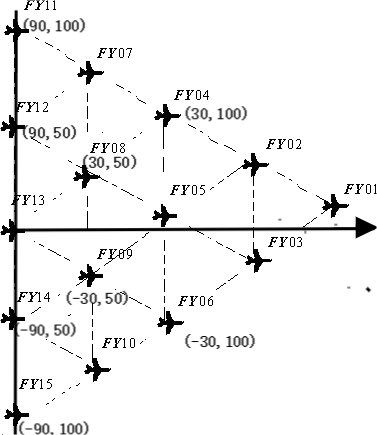
\includegraphics[height=5cm]{./figures/7-1.png}
		\caption{极坐标下的无人机锥形编队}\label{fig:15}
	\end{figure}
	
	(2)单位体系的约定:
	
	本题中,由于无人机编队的几何特征,部分无人机目标点的极轴长$\rho$、极角$\theta$为无理数,对程序运行的效率影响较大。故本题中考虑使用角度制避开无理数,同时只取轴长$\rho$小数后4位近似计算(在MATLAB中为short类型)。
	
	\subsubsection{默认“发射机”选择的调整}
	
	在章节6.3的队形调整模型中,默认选择了FA00、FA01号无人机作为“发射机”;本题中由于极心、队形改变,需要调整默认“发射机”。结合圆形编队下的“发射机”选取,我们考虑以FA13号无人机作为领航“发射机”,再仿照章节6.3.3新增“发射机的选取方式”,先确定2架无人机与FY13号机组成机队定位网络。
	
	%		\subsection{通过无人机的坐标系反推定无人机的坐标}
	%				
	%					\begin{equation}
	%							\tag{7-1-1}
	%							\begin{split}
	%							  \mid F_{05}F_{09}\mid = \sqrt{\rho_{5}^{2}+\rho_{9}^{2}} \\\mid F_{01}F_{03}\mid = \sqrt{\rho_{5}^{1}+\rho_{3}^{2}}
	%							\end{split}
	%					\end{equation}
	%							\begin{figure}[htbp!]
	%							\centering
	%							\captionsetup{font={small}}
	%							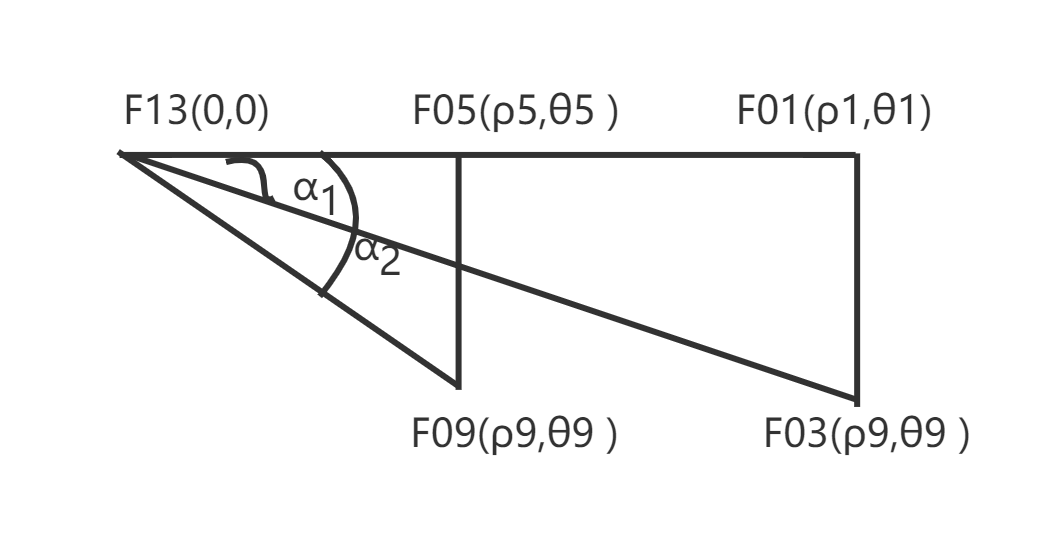
\includegraphics[height=5cm]{./figures/7-2.png}
	%							\caption{无人机锥形队极坐标演示图}\label{fig:16}
	%						\end{figure}
	\subsection{三点定位法原理及模型运用}
	
	在章节7.1.2中,我们选取了3架无人机作为信号“发射机”,由于选取的2架“发射机”可能有偏差,且本题中需要根据3点坐标解算其余12点坐标,对模型的可适用性要求较大。由于章节6.3中描述的圆心编队调整法使用到章节6.1中的圆形编队“接收机”定位模型;经过试验,我们发现6.1的定位模型在本题运用中效果不佳。
	
	已知选取的三架“发射机”到被观测机之间的相对关系,我们考虑使用“\textbf{三点定位法}”对受探无人机的坐标进行解算。“三点定位法”的原理如下:
	
	
	\noindent	\textbf{Step.1}绘制共弦双子圆:
	
	已选取三架“发射机”,记为:$A$、$B$、$C$,需检测一“接收机”$D$,假设四点不构成矩形,及四点不共圆,一定能画出一组以其中两点连线为公共弦的双圆,如图所示,由勾股定理可得方程组:
	\begin{figure}[htbp!]
		\centering
		\captionsetup{font={small}}
		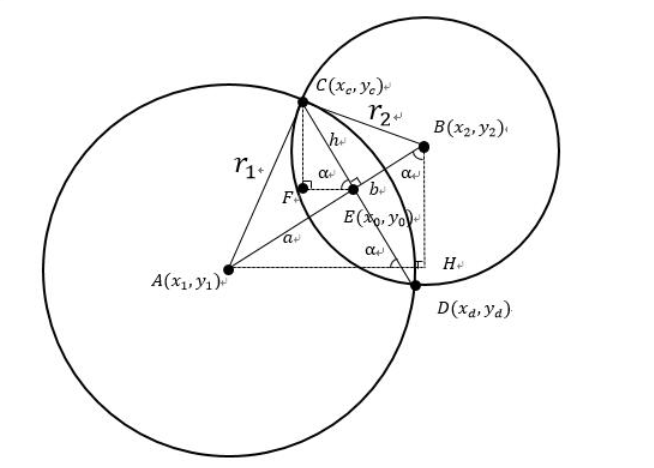
\includegraphics[height=5cm]{./figures/7-4.png}
		\caption{三点定位法示意图}\label{fig:17}
	\end{figure}
	\begin{equation}
		\tag{7-3-1}
		\left\{
		\begin{split}
			a^{2}+h^{2} =r_{1}^{2} \\
			b^{2}+h^{2} =r_{2}^{2} \\
			a+b = \rho_{ab}
		\end{split}\right
	\end{equation}
	
	根据式7-3-1,可以解得a:
	\begin{equation}
		\tag{7-3-2}
		a = \frac{r_{1}^{2}-r_{2}^{2}+\rho_{ab}^{2}}{2\rho_{ab}}
	\end{equation}
	
	\noindent	\textbf{Step.2}建立极坐标与直角坐标之间的关系:
	
	\begin{equation}
		\tag{7-3-3}
		\left\{
		\begin{split}
			x  = \rho+ r cos\theta \\
			y = \rho + r sin\theta \\
		\end{split}\right
	\end{equation}
	
	\noindent	\textbf{Step.3}计算受测点坐标:
	
	\begin{equation}
		\tag{7-3-4}
		\left\{
		\begin{split}
			x_{c} = x_{0} - \frac{h}{d}(y_{2}-y_{1}) \\
			y_{c} = x_{0} - \frac{h}{d}(x_{2}-x_{1}) \\
		\end{split}\right
	\end{equation}
	\qquad\qquad	或
	\begin{equation}
		\tag{7-3-4}
		\left\{
		\begin{split}
			x_{d} = x_{0} + \frac{h}{d}(y_{2}-y_{1}) \\
			y_{d} = x_{0}  + \frac{h}{d}(x_{2}-x_{1}) \\
		\end{split}\right
	\end{equation}
	\subsection{改进的卡尔曼滤波算法}	
	
	
	在章节6.3中的研究中,运用传统的“卡尔曼滤波器”,我们对无人机圆形编队下队形的调整算法建立了模型。本题在该题的基础上变换了队形,其余条件均未改变。据此,我们尝试使用章节6.3中的模型改进,使之适用于锥形队形。
	
	在章节7.1与7.2中,本文在新背景下对坐标系构建与位置信息解算设计了“三点定位”模型。与章节6.3的考虑类似,由于初始状态有2架“发射机”存在偏差,定位精度无法完全保证。同理使用卡尔曼滤波算法,对观测无人机的位置信息进行损失值评估。此处的损失函数仍与式6-3-6保持一致。利用卡尔曼滤波算法对带扰动数据的处理优势,多次进行无人机位置的调整,最终无人机离标定点的误差会逐渐缩小。根据章节6.2的结论,当无偏“发射机”多余4架后,可以准确不搜索出所有“接收机”的极坐标。
	
	\section{模型的评价和改进}
	
	\subsection{模型的优点和不足}	
	
	\subsubsection{问题一的模型评价}
	
	\noindent{\textbf{(1)误差分析:}}
	
	问题一共划分为3个小问,其中针对(1)小问对无人机圆形编队时,“接收机”的定位模型中基于古典几何学进行了数学解析。由于本题中将无人机编队理想化为登高平面,与实际机队编排差别较大。而且(1)小问中暂不考虑“发射机”存在偏差。
	
	针对(2)小问,本题中采用全局搜索方法,通过设定损失函数进行遍历效果评估。由于损失函数的定义为经验公式,缺少一定的理论推敲。而损失函数为本题中的核函数,对“发射机”序号的预测有直接影响。
	
	针对(3)小问,本题运用卡尔曼滤波器结合损失函数,采用先预测再更新的流程,动态进行
	
	\noindent{\textbf{(2)模型优点:}}
	
	对于(1)小问,由于本题直接运用逻辑演绎还原题目的数学需求,最终得出的模型具有较为理想的拟合优度,通过计算机数据模拟验证出模型具有较高的置信水平。
	
	对于(2)小问,本模型使用了全局搜索方法,当检索到符合要求的最优方案时,模型就会收敛。对于实际的无人机集群协同,计算量较小,对无人机的平台算力要求较低。
	
	对于(3)小问,在本题中对无人机编队参数设定运用了卡尔曼滤波器。卡尔曼滤波器因其自身的优点:递归运算、计算简单、自适应性、前瞻性等,能够对随机干扰下的线性动态系统进行最优估计,因而有着广泛的应用。
	
	\noindent{\textbf{(3)模型不足:}}
	
	对于(1)小问,本模型中对问题的理想化背景依赖较大,如果“发射机”没有沿着圆周均匀分布,那么模型的定位效果将会产生较大的误差。本题中采用了思路最为简朴的分类讨论法,给出了四类外围无人机的分布情况,分别就四种情况再进行数学解析。本方法由于情况较多,导致模型分类过于复杂,同时计算量较大,对计算机性能和编程能力提出较高要求。
	
	对于(2)小问,本题中运用到了全局搜索和损失函数,当损失趋于最少时,由于全局搜索的弊端容易陷入局部最小。
	
	对于(3)小问,本题中主要使\textbf{卡尔曼滤波器}算法,使受控无人机经过多次调整最终落到目标坐标点上。由于本题中观测数据有一定的误差,当无人机位置长时间重合时,会导致目标失踪,样本点缺失。
	
	\subsubsection{问题二的模型评价}
	\noindent{\textbf{(1)误差分析:}} 
	
	问题二的模型是在章节6.3圆形编队调整模型下进行改进而得。误差来源包括前验估计时直接假设了当前选中点近似在圆周上。此时,3架“发射机”监测的无人机坐标信息并不完全准确
	
	\noindent{\textbf{(2)模型优点:}} 
	
	本题的模型基于前述研究加以改进,模型的可靠性得到了一定验证。使用卡尔曼滤波器算法,对于有一定扰动范围的原始数据,可以实现效果良好的序号辨别。
	
	\noindent{\textbf{(3)模型不足:}} 
	
	问题二中根据无人机编队的布局特点建立的\textbf{三圆定位法},由于编队布局的对称性、对于同一组参考点和受观测点,模型可能推演出多组坐标。同时,由于本模型在设计定位算法时,对“发射机”内部存在受观测“接收机”等情况缺少细化考虑,在编程实现时依赖于大量分类讨论,使得代码逻辑过于冗杂,计算量增大。
	
	同时,对于三架“发射机”与观测的“接收机”正好处于四点共圆的情况,三圆定位发对坐标的确定就会失效。
	
	\subsection{模型的改进}	
	
	\subsubsection{问题一的模型改进}
	
	\textbf{对于(1)小问:\quad}本问中主要以几何学的解析法,分别对四种无人机位置情况进行几何演算;不妨考虑在本题中四类模型的基础上进行\textbf{二次抽象},利用圆周上三角形的性质、三角函数周期性等再做归纳,使无人机的位置分类减少。
	
	\textbf{对于(2)小问:\quad}本题中使用全局搜索法或导致局部最优,可以参考文献\cite{singer2009nelder}中引述Nelder\_Mead单纯形方法。
	
	\textbf{对于(3)小问:\quad} 本题就章节6.2模型进行改进,由于损失函数的使用存在一定的主观性,可以使用文献\cite{cai2018exploring}的中心损失(Center Loss)、文献\cite{deng2019arcface}的附加边角损失(AAMS)等方法对损失函数进行改进。
	\subsubsection{问题二的模型改进}	
	
	为了纠正问题二模型的多解问题,我们在模型中以增加字段的方式标明了受观测无人机相对于对称轴的关系。对于少数观测点,这种方法有可取之处,但当观测点
	数量达到一定规模后,增加数据维度容易陷入数维灾。针对对称问题,可以考虑使用"向量"方法解析坐标点的方向。
	
	对于“发射机”和“接受机”的相对关系问题,可以考虑用使用二分类法、调整极心等方法进行使点位置情况尽量减少;对于“四点共圆”问题,可以考虑通过缩小可行解范围,从多个可疑坐标中找出最符合要求的定位信息。
	\newpage
	\bibliography{bib/cite.bib}
	\newpage
	\begin{appendices}
		\section{文件列表}
		% Table generated by Excel2LaTeX from sheet 'Sheet1'
		\begin{table*}[htbp]
			\renewcommand\arraystretch{0.1}
			\tabcolsep=0.2cm
			\centering
			\caption{支撑材料列表清单(一)}
			\begin{tabular}{ccc}
				\toprule[1.5pt]
				\makebox[0.27\textwidth][c]{文件夹名}	& \makebox[0.3\textwidth][c]{文件夹内容}	& \makebox[0.4\textwidth][c]{文件描述} \\ 
				\midrule
				code1.1	& & 问题一(1)程序集 \\
				&code\_1\_1.m  & 1.1程序 \\
				
				&main\_fun.m  & 主函数\\
				
				&judge.m  & 解集极角整理\\
				
				&trans.m  & 弧度角度转换 \\
				&arg.m & 求$\alpha_{1}$、$\alpha_{2}$ 、$\alpha_{3}$  \\
				&model1.m  & 情况一 \\
				&model2.m  & 情况二 \\
				&model3.m  & 情况三 \\
				&model4.m  & 情况四 \\
				&location.mat  & 1.1程序数据 \\
				
				code1.2	&& 问题一(2)程序集 \\
				
				&code\_1\_2.m  & 1.2程序 \\
				
				&main\_fun.m  & 主函数\\
				
				&judge.m  & 解集极角整理\\
				
				&trans.m  & 弧度角度转换 \\
				&arg.m & 求$\alpha_{1}$、$\alpha_{2}$ 、$\alpha_{3}$  \\
				&model1.m  & 情况一 \\
				&model2.m  & 情况二 \\
				&model3.m  & 情况三 \\
				&model4.m  & 情况四 \\
				
				\bottomrule
			\end{tabular}%
			\label{tab:addlabel}%
		\end{table*}%
		\begin{table*}[htbp]
			\renewcommand\arraystretch{0.1}
			\tabcolsep=0.2cm
			\centering
			\caption{支撑材料列表清单(二)}
			\begin{tabular}{ccc}
				\toprule[1.5pt]
				\makebox[0.27\textwidth][c]{文件夹名}	& \makebox[0.3\textwidth][c]{文件夹内容}	& \makebox[0.4\textwidth][c]{文件描述} \\ 
				\midrule
				&loss\_fun1.m  & 新增1架损失函数\\
				&loss\_fun2.m  & 新增2架损失函数\\
				&location.mat  & 新增1架“发射机”数据 \\
				&location2.mat  & 新增2架“发射机”数据 \\
				code1.3	& & 问题一(3)程序集 \\
				code2	& & 问题二程序集 \\
				\bottomrule
			\end{tabular}%
			\label{tab:addlabel}%
		\end{table*}%
		
		% Please add the following required packages to your document preamble:
		% \usepackage{booktabs}
		
		\section{问题一(1)小问——MATLAB源程序}
		main\_fun.m
		\lstinputlisting[language=matlab]{code/1.1/main\_fun.m}
		code\_1\_1.m
		\lstinputlisting[language=matlab]{code/1.1/code\_1\_1.m}	
		trans.m
		\lstinputlisting[language=matlab]{code/1.1/trans.m}
		model1.m
		\lstinputlisting[language=matlab]{code/1.1/model1.m}
		model2.m
		\lstinputlisting[language=matlab]{code/1.1/model2.m}
		model3.m
		\lstinputlisting[language=matlab]{code/1.1/model3.m}
		model4.m
		\lstinputlisting[language=matlab]{code/1.1/model4.m}
		judge.m
		\lstinputlisting[language=matlab]{code/1.1/judge.m}
		arg.m
		\lstinputlisting[language=matlab]{code/1.1/arg.m}
		\section{问题一(2)小问——MATLAB源程序}
		main\_fun.m
		\lstinputlisting[language=matlab]{code/1.2/main\_fun.m}
		code\_1\_2.m
		\lstinputlisting[language=matlab]{code/1.2/code\_1\_2.m}
		loss\_fun1.m
		\lstinputlisting[language=matlab]{code/1.2/loss\_fun1.m}
		loss\_fun2.m
		\lstinputlisting[language=matlab]{code/1.2/loss\_fun2.m}
		trans.m
		\lstinputlisting[language=matlab]{code/1.2/trans.m}
		model1.m
		\lstinputlisting[language=matlab]{code/1.2/model1.m}
		model2.m
		\lstinputlisting[language=matlab]{code/1.2/model2.m}
		model3.m
		\lstinputlisting[language=matlab]{code/1.2/model3.m}
		model4.m
		\lstinputlisting[language=matlab]{code/1.2/model4.m}
		\section{问题一(3)小问——MATLAB源程序}
		
		\section{问题二——MATLAB源程序}	
		\section{附表:问题结果表格}
		
		% Please add the following required packages to your document preamble:
		% \usepackage{booktabs}
		\begin{table}[htbp!]
			\captionsetup{font={small}}
			\caption{问题一(1)问“接收机”定位模型验证数据表(1-35)}
			\footnotesize
			\centering
			\begin{tabular}{@{}ccccccccc@{}}
				\toprule
				\textbf{接收机编号} & \textbf{发射机编号} & \textbf{a1} & \textbf{a2} & \textbf{a3} & \textbf{真实位置极径} & \textbf{真实位置极角} & \textbf{模型输出极径} & \textbf{模型输出极角} \\ \midrule
				6              & 7              & 28.8594     & 66.2404     & 95.0998     & 105.2242        & 239.3820        & 105.2242        & 239.3820        \\
				2              & 3              & 50.9066     & 72.2338     & 21.3272     & 97.0403         & 80.2295         & 97.0403         & 80.2295         \\
				4              & 6              & 10.1527     & 47.9040     & 58.0567     & 105.1239        & 200.8316        & 105.1239        & 200.8316        \\
				9              & 3              & 48.8287     & 29.3571     & 19.4715     & 103.0628        & 80.2937         & 103.0628        & 80.2937         \\
				6              & 8              & 50.0504     & 49.6488     & 99.6993     & 100.4413        & 280.4038        & 100.4413        & 280.4038        \\
				2              & 3              & 47.2977     & 63.4888     & 16.1911     & 108.8599        & 79.5724         & 108.8599        & 79.5724         \\
				6              & 2              & 72.1601     & 9.7031      & 81.8632     & 97.8389         & 39.1946         & 97.8389         & 39.1946         \\
				5              & 7              & 29.7529     & 49.3822     & 79.1351     & 101.7220        & 240.0714        & 101.7220        & 240.0714        \\
				8              & 2              & 69.5583     & 29.8101     & 39.7482     & 100.4087        & 40.2456         & 100.4087        & 40.2456         \\
				5              & 8              & 51.3596     & 30.7755     & 82.1350     & 95.8703         & 279.8482        & 95.8703         & 279.8482        \\
				4              & 3              & 48.0136     & 66.5948     & 114.6083    & 104.8455        & 80.7881         & 104.8455        & 80.7881         \\
				4              & 9              & 74.8575     & 9.9702      & 64.8873     & 93.4453         & 319.2809        & 93.4453         & 319.2809        \\
				5              & 4              & 31.4936     & 75.2594     & 106.7530    & 93.0630         & 119.4177        & 93.0630         & 119.4177        \\
				7              & 5              & 10.5227     & 53.1322     & 63.6548     & 91.0751         & 159.9031        & 91.0751         & 159.9031        \\
				9              & 5              & 10.0082     & 9.5130      & 19.5212     & 104.8538        & 159.4924        & 104.8538        & 159.4924        \\
				9              & 2              & 71.7108     & 50.6821     & 21.0287     & 97.7000         & 40.2184         & 97.7000         & 40.2184         \\
				5              & 6              & 10.2638     & 66.1730     & 76.4369     & 104.4494        & 200.9896        & 104.4494        & 200.9896        \\
				6              & 4              & 30.2154     & 49.7541     & 79.9695     & 100.0603        & 119.5491        & 100.0603        & 119.5491        \\
				8              & 9              & 64.0479     & 63.9690     & 128.0169    & 107.9435        & 320.1165        & 107.9435        & 320.1165        \\
				8              & 5              & 10.2159     & 30.8074     & 41.0233     & 95.3709         & 160.0459        & 95.3709         & 160.0459        \\
				9              & 6              & 10.1087     & 31.1118     & 21.0031     & 91.5979         & 199.3603        & 91.5979         & 199.3603        \\
				6              & 8              & 52.7512     & 52.4127     & 105.1638    & 92.7084         & 280.3101        & 92.7084         & 280.3101        \\
				3              & 4              & 30.2836     & 72.6572     & 42.3736     & 96.1740         & 120.7048        & 96.1740         & 120.7048        \\
				7              & 9              & 73.7526     & 51.8369     & 125.5895    & 95.1446         & 319.7388        & 95.1446         & 319.7388        \\
				2              & 6              & 10.2033     & 9.9566      & 20.1599     & 98.4301         & 200.2447        & 98.4301         & 200.2447        \\
				5              & 6              & 10.4505     & 76.0201     & 86.4706     & 92.5189         & 200.1114        & 92.5189         & 200.1114        \\
				5              & 7              & 30.1568     & 50.5086     & 80.6654     & 98.6964         & 239.8806        & 98.6964         & 239.8806        \\
				3              & 2              & 65.1180     & 65.6498     & 130.7679    & 106.0533        & 40.7087         & 106.0533        & 40.7087         \\
				4              & 6              & 9.6816      & 50.2898     & 59.9714     & 100.0726        & 199.3704        & 100.0726        & 199.3704        \\
				6              & 9              & 76.3443     & 31.8632     & 108.2075    & 91.5926         & 319.2218        & 91.5926         & 319.2218        \\
				8              & 7              & 29.7043     & 66.9311     & 37.2268     & 104.4514        & 240.8744        & 104.4514        & 240.8744        \\
				4              & 2              & 63.4247     & 47.5486     & 110.9733    & 108.4381        & 40.6892         & 108.4381        & 40.6892         \\
				8              & 5              & 9.8312      & 30.6855     & 40.5168     & 97.6396         & 160.5718        & 97.6396         & 160.5718        \\
				3              & 6              & 10.1385     & 28.9686     & 39.1070     & 104.2338        & 200.7110        & 104.2338        & 200.7110        \\ \bottomrule
			\end{tabular}
		\end{table}
		
		% Please add the following required packages to your document preamble:
		% \usepackage{booktabs}
		\begin{table}[htbp!]
			\captionsetup{font={small}}
			\caption{问题一(1)问“接收机”定位模型验证数据表(36-70)}
			\footnotesize
			\centering
			\centering
			\begin{tabular}{@{}ccccccccc@{}}
				\toprule
				\textbf{接收机编号} & \textbf{发射机编号} & \textbf{a1} & \textbf{a2} & \textbf{a3} & \textbf{真实位置极径} & \textbf{真实位置极角} & \textbf{模型输出极径} & \textbf{模型输出极角} \\ \midrule
				30.8601        & 74.3993        & 105.2594    & 94.6284     & 239.8981    & 94.6284         & 239.8981        & 105.2242        & 239.3820        \\
				30.8767        & 30.2710        & 61.1477     & 96.5897     & 119.4079    & 96.5897         & 119.4079        & 97.0403         & 80.2295         \\
				9.8188         & 10.3166        & 20.1355     & 98.6680     & 160.4944    & 98.6680         & 160.4944        & 105.1239        & 200.8316        \\
				9.2892         & 9.8890         & 19.1782     & 108.4790    & 160.6261    & 108.4790        & 160.6261        & 103.0628        & 80.2937         \\
				72.5181        & 71.4893        & 144.0075    & 97.4866     & 39.0721     & 97.4866         & 39.0721         & 100.4413        & 280.4038        \\
				9.2743         & 28.5997        & 19.3253     & 106.0870    & 160.8813    & 106.0870        & 160.8813        & 108.8599        & 79.5724         \\
				73.9024        & 10.3423        & 63.5601     & 95.2962     & 39.8069     & 95.2962         & 39.8069         & 97.8389         & 39.1946         \\
				10.7087        & 30.4647        & 41.1734     & 94.6940     & 200.8429    & 94.6940         & 200.8429        & 101.7220        & 240.0714        \\
				53.0919        & 30.9384        & 84.0303     & 92.3760     & 280.7074    & 92.3760         & 280.7074        & 100.4087        & 40.2456         \\
				51.3481        & 30.8193        & 20.5288     & 97.0685     & 280.6416    & 97.0685         & 280.6416        & 95.8703         & 279.8482        \\
				48.1489        & 65.4695        & 17.3205     & 106.1362    & 280.3895    & 106.1362        & 280.3895        & 104.8455        & 80.7881         \\
				9.9838         & 9.6358         & 19.6196     & 103.8373    & 159.6451    & 103.8373        & 159.6451        & 93.4453         & 319.2809        \\
				9.6981         & 49.2642        & 39.5661     & 101.5111    & 199.5441    & 101.5111        & 199.5441        & 93.0630         & 119.4177        \\
				63.1636        & 46.8488        & 110.0124    & 109.2568    & 39.7013     & 109.2568        & 39.7013         & 91.0751         & 159.9031        \\
				65.2281        & 65.1320        & 130.3601    & 106.3325    & 39.8701     & 106.3325        & 39.8701         & 104.8538        & 159.4924        \\
				9.8469         & 48.2065        & 38.3596     & 105.7861    & 159.7303    & 105.7861        & 159.7303        & 97.7000         & 40.2184         \\
				52.1725        & 31.0376        & 21.1349     & 93.7430     & 80.0586     & 93.7430         & 80.0586         & 104.4494        & 200.9896        \\
				51.4269        & 73.8647        & 22.4378     & 94.4892     & 279.0501    & 94.4892         & 279.0501        & 100.0603        & 119.5491        \\
				30.3128        & 74.4751        & 104.7879    & 95.1795     & 120.9763    & 95.1795         & 120.9763        & 107.9435        & 320.1165        \\
				51.8242        & 30.7177        & 82.5419     & 95.1116     & 280.2149    & 95.1116         & 280.2149        & 95.3709         & 160.0459        \\
				48.3323        & 29.9056        & 78.2379     & 103.5573    & 279.0094    & 103.5573        & 279.0094        & 91.5979         & 199.3603        \\
				51.5723        & 30.2396        & 81.8120     & 96.5000     & 280.6829    & 96.5000         & 280.6829        & 92.7084         & 280.3101        \\
				47.2764        & 10.0411        & 57.3175     & 107.1425    & 80.8077     & 107.1425        & 80.8077         & 96.1740         & 120.7048        \\
				29.5219        & 9.8344         & 19.6875     & 102.7586    & 239.9428    & 102.7586        & 239.9428        & 95.1446         & 319.7388        \\
				10.3550        & 53.4393        & 63.7943     & 90.7772     & 199.7458    & 90.7772         & 199.7458        & 98.4301         & 200.2447        \\
				9.9974         & 72.3637        & 62.3663     & 96.8101     & 199.6727    & 96.8101         & 199.6727        & 92.5189         & 200.1114        \\
				63.8131        & 47.4109        & 16.4022     & 108.3691    & 39.6647     & 108.3691        & 39.6647         & 98.6964         & 239.8806        \\
				9.9954         & 66.7669        & 76.7622     & 103.9806    & 200.3929    & 103.9806        & 200.3929        & 106.0533        & 40.7087         \\
				50.2675        & 50.7886        & 101.0561    & 98.4653     & 80.5116     & 98.4653         & 80.5116         & 100.0726        & 199.3704        \\
				74.4391        & 52.3593        & 126.7984    & 94.1018     & 319.4686    & 94.1018         & 319.4686        & 91.5926         & 319.2218        \\
				77.0990        & 31.1382        & 108.2373    & 91.7600     & 320.5353    & 91.7600         & 320.5353        & 104.4514        & 240.8744        \\
				63.1093        & 28.6416        & 34.4677     & 109.3067    & 320.2383    & 109.3067        & 320.2383        & 108.4381        & 40.6892         \\
				30.0742        & 10.5738        & 40.6480     & 97.0346     & 120.8307    & 97.0346         & 120.8307        & 97.6396         & 160.5718        \\
				49.7478        & 9.6232         & 59.3710     & 101.6092    & 79.4027     & 101.6092        & 79.4027         & 104.2338        & 200.7110        \\ \bottomrule
			\end{tabular}
		\end{table}
		
		
		
		% Please add the following required packages to your document preamble:
		% \usepackage{booktabs}
		\begin{table}[htbp!]
			\captionsetup{font={small}}
			\caption{问题一(1)问“接收机”定位模型验证数据表(71-102)}
			\footnotesize
			\centering
			\begin{tabular}{@{}ccccccccc@{}}
				\toprule
				\textbf{接收机编号} & \textbf{发射机编号} & \textbf{a1} & \textbf{a2} & \textbf{a3} & \textbf{真实位置极径} & \textbf{真实位置极角} & \textbf{模型输出极径} & \textbf{模型输出极角} \\ \midrule
				9              & 3              & 52.1501     & 31.0863     & 21.0637     & 94.1446         & 79.8294         & 94.1446         & 79.8294         \\
				8              & 2              & 71.6067     & 30.5925     & 41.0142     & 98.4116         & 39.3517         & 98.4116         & 39.3517         \\
				8              & 6              & 10.2059     & 51.8351     & 41.6292     & 94.5402         & 199.8491        & 94.5402         & 199.8491        \\
				8              & 7              & 29.3775     & 67.9828     & 38.6053     & 102.3030        & 239.5006        & 102.3030        & 239.5006        \\
				2              & 3              & 49.6583     & 68.8871     & 19.2288     & 101.7165        & 79.5112         & 101.7165        & 79.5112         \\
				5              & 3              & 49.7419     & 50.6547     & 100.3966    & 99.4209         & 80.9065         & 99.4209         & 80.9065         \\
				4              & 8              & 48.2407     & 9.7296      & 57.9703     & 105.3171        & 280.0181        & 105.3171        & 280.0181        \\
				3              & 2              & 78.2782     & 77.5173     & 155.7955    & 90.3889         & 39.4655         & 90.3889         & 39.4655         \\
				5              & 8              & 49.6289     & 30.1348     & 79.7637     & 100.4684        & 279.5744        & 100.4684        & 279.5744        \\
				2              & 9              & 65.1207     & 48.0437     & 17.0770     & 106.6806        & 320.5420        & 106.6806        & 320.5420        \\
				6              & 8              & 50.7000     & 50.2541     & 100.9541    & 98.6124         & 280.4384        & 98.6124         & 280.4384        \\
				2              & 6              & 10.0965     & 10.0301     & 20.1266     & 98.7548         & 200.0659        & 98.7548         & 200.0659        \\
				3              & 7              & 29.8097     & 9.3590      & 39.1687     & 103.9128        & 240.9123        & 103.9128        & 240.9123        \\
				2              & 4              & 31.3090     & 52.3874     & 21.0784     & 94.1029         & 119.4156        & 94.1029         & 119.4156        \\
				4              & 6              & 9.8738      & 48.2714     & 58.1453     & 104.8584        & 200.2326        & 104.8584        & 200.2326        \\
				7              & 2              & 77.0989     & 10.9329     & 66.1660     & 92.1257         & 39.0045         & 92.1257         & 39.0045         \\
				2              & 4              & 30.5337     & 51.1666     & 20.6328     & 96.4607         & 120.1214        & 96.4607         & 120.1214        \\
				2              & 7              & 28.9977     & 9.9285      & 19.0692     & 108.4054        & 240.7011        & 108.4054        & 240.7011        \\
				4              & 6              & 10.0825     & 47.1880     & 57.2705     & 107.2788        & 200.9075        & 107.2788        & 200.9075        \\
				7              & 2              & 76.4838     & 10.2462     & 66.2376     & 91.7662         & 40.3593         & 91.7662         & 40.3593         \\
				7              & 5              & 9.9731      & 48.6975     & 58.6706     & 103.4601        & 159.7051        & 103.4601        & 159.7051        \\
				6              & 4              & 29.5838     & 48.5523     & 78.1361     & 103.7551        & 119.6034        & 103.7551        & 119.6034        \\
				6              & 4              & 28.6017     & 47.0105     & 75.6123     & 109.0593        & 119.9259        & 109.0593        & 119.9259        \\
				9              & 5              & 9.4177      & 10.0949     & 19.5126     & 104.9438        & 160.6944        & 104.9438        & 160.6944        \\
				9              & 4              & 31.4429     & 10.2452     & 21.1976     & 90.0549         & 120.5378        & 90.0549         & 120.5378        \\
				7              & 9              & 71.3022     & 49.9158     & 121.2180    & 98.9395         & 320.8850        & 98.9395         & 320.8850        \\
				8              & 3              & 50.5128     & 10.2388     & 40.2740     & 99.0667         & 79.6190         & 99.0667         & 79.6190         \\
				7              & 8              & 47.5080     & 65.4719     & 112.9799    & 106.3555        & 279.1581        & 106.3555        & 279.1581        \\
				6              & 7              & 30.4903     & 75.1545     & 105.6447    & 94.3316         & 239.0863        & 94.3316         & 239.0863        \\
				8              & 4              & 29.2954     & 9.2199      & 38.5153     & 107.0983        & 119.1006        & 107.0983        & 119.1006        \\
				9              & 4              & 30.0656     & 10.0590     & 20.0066     & 99.9424         & 119.8879        & 99.9424         & 119.8879        \\ \bottomrule
			\end{tabular}
		\end{table}
		
		
		% Please add the following required packages to your document preamble:
		% \usepackage{booktabs}
		\begin{table}[htbp!]
			\footnotesize
			\captionsetup{font={small}}
			\caption{问题一(2)问“接收机”定位模型验证数据表(1-35)}
			\centering
			%					\renewcommand\arraystretch{4}
			\tabcolsep=0.1cm
			\begin{tabular}{@{}cccccccccc@{}}
				\toprule
				\multicolumn{3}{c}{\textbf{FYX1发射机对应的发射角}}                                                           & \multicolumn{3}{c}{\textbf{FYX2发射机对应的发射角}}                                                           & \textbf{FYX1的真实编号} & \textbf{FYX2的真实编号} & \textbf{FYX1模型识别编号} & \textbf{FYX2模型识别编号} \\ \midrule
				\multicolumn{1}{c|}{\textbf{$\alpha_{1}$}} & \multicolumn{1}{c|}{\textbf{$\alpha_{2}$}} & \multicolumn{1}{c|}{\textbf{$\alpha_{3}$}} & \multicolumn{1}{c|}{\textbf{$\alpha_{1}$}} & \multicolumn{1}{c|}{\textbf{$\alpha_{2}$}} & \multicolumn{1}{c|}{\textbf{$\alpha_{3}$}} & \multicolumn{4}{c}{\textbf{}}  
				\\ \midrule
				9.7917                           & 52.1907                          & 61.9825                          & 9.7917                           & 31.2953                          & 41.0871                          & 7                    & 8                    & 7                      & 8                      \\
				66.6277                          & 29.8035                          & 96.4311                          & 66.6277                          & 9.3708                           & 57.2568                          & 5                    & 7                    & 5                      & 7                      \\
				46.5893                          & 62.7189                          & 16.1296                          & 46.5893                          & 28.8778                          & 75.4670                          & 2                    & 6                    & 2                      & 6                      \\
				30.8234                          & 75.4210                          & 44.5976                          & 30.8234                          & 10.8140                          & 41.6374                          & 3                    & 8                    & 3                      & 8                      \\
				65.1491                          & 64.9471                          & 130.0962                         & 65.1491                          & 9.8149                           & 55.3343                          & 3                    & 7                    & 3                      & 7                      \\
				64.9607                          & 28.6424                          & 36.3183                          & 64.9607                          & 47.5875                          & 17.3732                          & 8                    & 9                    & 8                      & 9                      \\
				65.1266                          & 48.1506                          & 16.9760                          & 65.1266                          & 29.3292                          & 35.7974                          & 2                    & 3                    & 2                      & 3                      \\
				30.8349                          & 30.7603                          & 61.5951                          & 30.8349                          & 51.6842                          & 20.8493                          & 4                    & 9                    & 4                      & 9                      \\
				53.1828                          & 78.4849                          & 131.6677                         & 53.1828                          & 10.8320                          & 64.0148                          & 4                    & 7                    & 4                      & 7                      \\
				48.2132                          & 10.1367                          & 38.0765                          & 48.2132                          & 47.3229                          & 95.5361                          & 3                    & 6                    & 3                      & 6                      \\
				10.4827                          & 49.6887                          & 60.1714                          & 10.4827                          & 50.6123                          & 40.1297                          & 4                    & 8                    & 4                      & 8                      \\
				50.1945                          & 71.3431                          & 121.5376                         & 50.1945                          & 9.8035                           & 40.3911                          & 4                    & 8                    & 4                      & 8                      \\
				10.2994                          & 53.2190                          & 63.5184                          & 10.2994                          & 77.2202                          & 87.5196                          & 4                    & 5                    & 4                      & 5                      \\
				77.5701                          & 10.5278                          & 67.0424                          & 77.5701                          & 53.3196                          & 24.2506                          & 7                    & 9                    & 7                      & 9                      \\
				52.1252                          & 30.9075                          & 21.2176                          & 52.1252                          & 75.1694                          & 23.0443                          & 2                    & 9                    & 2                      & 9                      \\
				69.8946                          & 29.6418                          & 40.2528                          & 69.8946                          & 49.7142                          & 20.1804                          & 8                    & 9                    & 8                      & 9                      \\
				64.3400                          & 28.5753                          & 35.7647                          & 64.3400                          & 64.7468                          & 129.0869                         & 3                    & 8                    & 3                      & 8                      \\
				48.4272                          & 49.3595                          & 97.7867                          & 48.4272                          & 28.9892                          & 19.4380                          & 5                    & 9                    & 5                      & 9                      \\
				69.3362                          & 29.5484                          & 98.8846                          & 69.3362                          & 9.6812                           & 79.0174                          & 5                    & 6                    & 5                      & 6                      \\
				28.3972                          & 9.3196                           & 19.0776                          & 28.3972                          & 9.8660                           & 38.2632                          & 2                    & 3                    & 2                      & 3                      \\
				30.0556                          & 29.0744                          & 59.1300                          & 30.0556                          & 10.3597                          & 19.6959                          & 7                    & 9                    & 7                      & 9                      \\
				71.5120                          & 50.4069                          & 21.1051                          & 71.5120                          & 51.3404                          & 122.8524                         & 2                    & 7                    & 2                      & 7                      \\
				52.2194                          & 30.9319                          & 21.2875                          & 52.2194                          & 75.4319                          & 23.2125                          & 2                    & 9                    & 2                      & 9                      \\
				67.4398                          & 9.7901                           & 77.2299                          & 67.4398                          & 9.8763                           & 57.5636                          & 6                    & 7                    & 6                      & 7                      \\
				10.0599                          & 50.6557                          & 40.5959                          & 10.0599                          & 10.1473                          & 20.2072                          & 3                    & 9                    & 3                      & 9                      \\
				10.1855                          & 31.4205                          & 41.6060                          & 10.1855                          & 31.0369                          & 20.8513                          & 3                    & 9                    & 3                      & 9                      \\
				53.0651                          & 10.5410                          & 63.6061                          & 53.0651                          & 77.3187                          & 130.3839                         & 4                    & 7                    & 4                      & 7                      \\
				53.0107                          & 52.6836                          & 105.6944                         & 53.0107                          & 10.2666                          & 63.2773                          & 5                    & 7                    & 5                      & 7                      \\
				30.0523                          & 50.3392                          & 80.3915                          & 30.0523                          & 10.1143                          & 40.1666                          & 6                    & 8                    & 6                      & 8                      \\
				66.9684                          & 67.0424                          & 134.0108                         & 66.9684                          & 9.7643                           & 57.2040                          & 3                    & 7                    & 3                      & 7                      \\
				9.4760                           & 63.1635                          & 53.6876                          & 9.4760                           & 28.6550                          & 38.1309                          & 4                    & 8                    & 4                      & 8                      \\
				68.9894                          & 69.3591                          & 138.3485                         & 68.9894                          & 29.6343                          & 39.3551                          & 3                    & 8                    & 3                      & 8                      \\ \bottomrule
			\end{tabular}
		\end{table}
		
		
		% Please add the following required packages to your document preamble:
		% \usepackage{booktabs}
		\begin{table}[htbp!]
			\footnotesize
			\captionsetup{font={small}}
			\caption{问题一(2)问“接收机”定位模型验证数据表(36-70)}
			\centering
			%					\renewcommand\arraystretch{4}
			\tabcolsep=0.1cm
			\begin{tabular}{@{}cccccccccc@{}}
				\toprule
				\multicolumn{3}{c}{\textbf{FYX1发射机对应的发射角}}                                                           & \multicolumn{3}{c}{\textbf{FYX2发射机对应的发射角}}                                                           & \textbf{FYX1的真实编号} & \textbf{FYX2的真实编号} & \textbf{FYX1模型识别编号} & \textbf{FYX2模型识别编号} \\ \midrule
				\multicolumn{1}{c|}{\textbf{$\alpha_{1}$}} & \multicolumn{1}{c|}{\textbf{$\alpha_{2}$}} & \multicolumn{1}{c|}{\textbf{$\alpha_{3}$}} & \multicolumn{1}{c|}{\textbf{$\alpha_{1}$}} & \multicolumn{1}{c|}{\textbf{$\alpha_{2}$}} & \multicolumn{1}{c|}{\textbf{$\alpha_{3}$}} & \multicolumn{4}{c}{\textbf{}}  
				\\ \midrule
				50.5201                          & 30.4432                          & 80.9633                          & 50.5201                          & 50.7795                          & 101.2996                         & 5                    & 6                    & 5                      & 6                      \\
				66.2917                          & 10.2523                          & 76.5440                          & 66.2917                          & 9.3215                           & 56.9702                          & 6                    & 7                    & 6                      & 7                      \\
				70.2059                          & 70.3136                          & 140.5195                         & 70.2059                          & 30.1078                          & 100.3137                         & 3                    & 5                    & 3                      & 5                      \\
				52.0330                          & 30.8477                          & 21.1853                          & 52.0330                          & 31.3999                          & 83.4329                          & 2                    & 5                    & 2                      & 5                      \\
				31.0110                          & 30.6212                          & 61.6322                          & 31.0110                          & 73.6499                          & 104.6610                         & 4                    & 6                    & 4                      & 6                      \\
				64.9693                          & 29.1587                          & 35.8106                          & 64.9693                          & 9.4014                           & 74.3707                          & 3                    & 5                    & 3                      & 5                      \\
				49.8079                          & 30.0401                          & 19.7678                          & 49.8079                          & 9.6768                           & 59.4848                          & 2                    & 4                    & 2                      & 4                      \\
				52.7032                          & 31.2986                          & 84.0018                          & 52.7032                          & 76.1839                          & 128.8871                         & 5                    & 7                    & 5                      & 7                      \\
				53.5358                          & 10.2354                          & 63.7711                          & 53.5358                          & 53.0061                          & 106.5419                         & 4                    & 6                    & 4                      & 6                      \\
				75.7802                          & 9.9006                           & 85.6807                          & 75.7802                          & 31.5441                          & 44.2361                          & 6                    & 8                    & 6                      & 8                      \\
				28.9008                          & 64.8889                          & 35.9881                          & 28.9008                          & 64.9294                          & 93.8302                          & 3                    & 5                    & 3                      & 5                      \\
				10.3693                          & 73.1151                          & 83.4844                          & 10.3693                          & 51.5933                          & 41.2239                          & 5                    & 8                    & 5                      & 8                      \\
				47.6548                          & 28.8776                          & 18.7772                          & 47.6548                          & 64.5675                          & 16.9127                          & 2                    & 9                    & 2                      & 9                      \\
				66.7528                          & 10.2127                          & 56.5400                          & 66.7528                          & 48.0011                          & 114.7539                         & 4                    & 7                    & 4                      & 7                      \\
				10.1278                          & 72.8613                          & 82.9890                          & 10.1278                          & 51.2698                          & 61.3975                          & 6                    & 7                    & 6                      & 7                      \\
				9.8947                           & 67.0116                          & 57.1169                          & 9.8947                           & 66.8555                          & 76.7503                          & 4                    & 6                    & 4                      & 6                      \\
				9.9563                           & 68.3176                          & 58.3613                          & 9.9563                           & 9.8196                           & 19.7760                          & 4                    & 9                    & 4                      & 9                      \\
				10.4588                          & 74.3588                          & 63.9001                          & 10.4588                          & 31.0638                          & 20.6050                          & 7                    & 9                    & 7                      & 9                      \\
				9.7239                           & 28.3083                          & 38.0322                          & 9.7239                           & 62.7326                          & 72.4565                          & 3                    & 5                    & 3                      & 5                      \\
				29.4295                          & 68.8252                          & 98.2547                          & 29.4295                          & 49.6486                          & 79.0782                          & 5                    & 6                    & 5                      & 6                      \\
				66.6716                          & 48.3540                          & 18.3176                          & 66.6716                          & 9.4703                           & 57.2013                          & 2                    & 4                    & 2                      & 4                      \\
				46.9737                          & 63.0295                          & 16.0557                          & 46.9737                          & 9.5644                           & 37.4093                          & 2                    & 8                    & 2                      & 8                      \\
				29.5692                          & 9.3069                           & 38.8761                          & 29.5692                          & 66.2653                          & 36.6962                          & 3                    & 8                    & 3                      & 8                      \\
				62.4825                          & 28.6751                          & 91.1576                          & 62.4825                          & 47.0088                          & 109.4914                         & 6                    & 7                    & 6                      & 7                      \\
				51.1955                          & 10.4058                          & 40.7898                          & 51.1955                          & 30.1757                          & 81.3712                          & 3                    & 5                    & 3                      & 5                      \\
				31.2545                          & 10.3237                          & 41.5782                          & 31.2545                          & 52.4459                          & 83.7003                          & 3                    & 5                    & 3                      & 5                      \\
				10.0369                          & 10.0262                          & 20.0631                          & 10.0369                          & 50.2185                          & 40.1816                          & 2                    & 8                    & 2                      & 8                      \\
				10.4499                          & 31.5853                          & 42.0352                          & 10.4499                          & 77.3434                          & 66.8935                          & 3                    & 7                    & 3                      & 7                      \\
				52.8385                          & 76.9032                          & 24.0647                          & 52.8385                          & 77.8348                          & 130.6733                         & 2                    & 4                    & 2                      & 4                      \\
				77.5268                          & 10.2141                          & 87.7408                          & 77.5268                          & 31.2661                          & 108.7929                         & 5                    & 6                    & 5                      & 6                      \\ \cmidrule(lr){7-7}
				48.6882                          & 28.7307                          & 77.4189                          & 48.6882                          & 65.6647                          & 114.3529                         & 5                    & 7                    & 5                      & 7                      \\
				68.7690                          & 67.9336                          & 136.7026                         & 68.7690                          & 29.2013                          & 97.9702                          & 3                    & 5                    & 3                      & 5                      \\
				50.0602                          & 71.1311                          & 121.1912                         & 50.0602                          & 9.7577                           & 40.3025                          & 4                    & 8                    & 4                      & 8                      \\
				65.3320                          & 10.0084                          & 55.3236                          & 65.3320                          & 48.1745                          & 17.1575                          & 7                    & 9                    & 7                      & 9                      \\
				63.7404                          & 47.2366                          & 16.5039                          & 63.7404                          & 9.5377                           & 54.2027                          & 2                    & 4                    & 2                      & 4                      \\
				72.7460                          & 9.9916                           & 62.7544                          & 72.7460                          & 30.4247                          & 42.3213                          & 7                    & 8                    & 7                      & 8                      \\
				76.4732                          & 52.7686                          & 23.7046                          & 76.4732                          & 31.2918                          & 45.1813                          & 2                    & 3                    & 2                      & 3                      \\
				70.3277                          & 9.8705                           & 80.1982                          & 70.3277                          & 30.1803                          & 40.1474                          & 6                    & 8                    & 6                      & 8                      \\
				48.2595                          & 66.1713                          & 17.9118                          & 48.2595                          & 29.3429                          & 77.6024                          & 2                    & 6                    & 2                      & 6                      \\
				76.1101                          & 31.4613                          & 44.6488                          & 76.1101                          & 52.2850                          & 128.3950                         & 3                    & 7                    & 3                      & 7                      \\ \bottomrule
			\end{tabular}
		\end{table}
		
		\begin{table}[htbp!]
			\footnotesize
			\captionsetup{font={small}}
			\caption{问题一(2)问“接收机”定位模型验证数据表(71-100)}
			\centering
			%					\renewcommand\arraystretch{4}
			\tabcolsep=0.1cm
			\begin{tabular}{@{}cccccccccc@{}}
				\toprule
				\multicolumn{3}{c}{\textbf{FYX1发射机对应的发射角}}                                                           & \multicolumn{3}{c}{\textbf{FYX2发射机对应的发射角}}                                                           & \textbf{FYX1的真实编号} & \textbf{FYX2的真实编号} & \textbf{FYX1模型识别编号} & \textbf{FYX2模型识别编号} \\ \midrule
				\multicolumn{1}{c|}{\textbf{$\alpha_{1}$}} & \multicolumn{1}{c|}{\textbf{$\alpha_{2}$}} & \multicolumn{1}{c|}{\textbf{$\alpha_{3}$}} & \multicolumn{1}{c|}{\textbf{$\alpha_{1}$}} & \multicolumn{1}{c|}{\textbf{$\alpha_{2}$}} & \multicolumn{1}{c|}{\textbf{$\alpha_{3}$}} & \multicolumn{4}{c}{\textbf{}}  
				\\ \midrule                                
				72.7460                          & 9.9916                           & 62.7544                          & 72.7460                          & 30.4247                          & 42.3213                          & 7                    & 8                    & 7                      & 8                      \\
				76.4732                          & 52.7686                          & 23.7046                          & 76.4732                          & 31.2918                          & 45.1813                          & 2                    & 3                    & 2                      & 3                      \\
				70.3277                          & 9.8705                           & 80.1982                          & 70.3277                          & 30.1803                          & 40.1474                          & 6                    & 8                    & 6                      & 8                      \\
				48.2595                          & 66.1713                          & 17.9118                          & 48.2595                          & 29.3429                          & 77.6024                          & 2                    & 6                    & 2                      & 6                      \\
				76.1101                          & 31.4613                          & 44.6488                          & 76.1101                          & 52.2850                          & 128.3950                         & 3                    & 7                    & 3                      & 7                      \\
				10.1918                          & 9.6688                           & 19.8606                          & 10.1918                          & 68.6661                          & 78.8579                          & 2                    & 5                    & 2                      & 5                      \\
				64.9630                          & 29.3032                          & 94.2662                          & 64.9630                          & 47.6143                          & 17.3487                          & 5                    & 9                    & 5                      & 9                      \\
				49.1330                          & 68.2604                          & 19.1275                          & 49.1330                          & 68.6158                          & 117.7487                         & 2                    & 4                    & 2                      & 4                      \\
				46.3829                          & 9.1169                           & 37.2660                          & 46.3829                          & 62.8120                          & 109.1949                         & 3                    & 7                    & 3                      & 7                      \\
				9.5648                           & 28.7928                          & 19.2281                          & 9.5648                           & 64.7890                          & 74.3537                          & 2                    & 6                    & 2                      & 6                      \\
				70.6325                          & 9.6176                           & 80.2501                          & 70.6325                          & 10.4121                          & 60.2205                          & 6                    & 7                    & 6                      & 7                      \\
				10.2473                          & 49.9486                          & 39.7014                          & 10.2473                          & 69.4848                          & 59.2376                          & 3                    & 4                    & 3                      & 4                      \\
				63.1109                          & 28.8817                          & 34.2292                          & 63.1109                          & 46.5191                          & 109.6300                         & 3                    & 7                    & 3                      & 7                      \\
				48.9933                          & 48.9024                          & 97.8957                          & 48.9933                          & 9.7978                           & 58.7911                          & 5                    & 7                    & 5                      & 7                      \\
				65.9427                          & 10.1549                          & 55.7877                          & 65.9427                          & 65.2557                          & 131.1983                         & 4                    & 8                    & 4                      & 8                      \\
				75.1548                          & 74.2329                          & 149.3877                         & 75.1548                          & 31.3704                          & 43.7843                          & 3                    & 8                    & 3                      & 8                      \\
				71.6527                          & 29.9916                          & 101.6443                         & 71.6527                          & 50.8766                          & 20.7761                          & 5                    & 9                    & 5                      & 9                      \\
				77.3903                          & 53.9233                          & 131.3136                         & 77.3903                          & 78.5381                          & 155.9284                         & 7                    & 8                    & 7                      & 8                      \\
				48.1983                          & 28.9225                          & 77.1208                          & 48.1983                          & 47.9289                          & 96.1272                          & 5                    & 6                    & 5                      & 6                      \\
				74.9101                          & 75.9870                          & 150.8971                         & 74.9101                          & 31.5832                          & 106.4932                         & 3                    & 5                    & 3                      & 5                      \\
				10.3386                          & 29.7594                          & 40.0980                          & 10.3386                          & 50.4719                          & 40.1333                          & 3                    & 8                    & 3                      & 8                      \\
				10.3398                          & 68.4400                          & 58.1002                          & 10.3398                          & 49.5990                          & 39.2592                          & 7                    & 8                    & 7                      & 8                      \\
				52.9097                          & 75.4846                          & 128.3944                         & 52.9097                          & 10.7072                          & 42.2026                          & 4                    & 8                    & 4                      & 8                      \\
				30.8286                          & 73.7353                          & 42.9067                          & 30.8286                          & 51.6514                          & 20.8228                          & 8                    & 9                    & 8                      & 9                      \\
				52.6334                          & 76.6144                          & 23.9810                          & 52.6334                          & 32.0583                          & 84.6916                          & 2                    & 6                    & 2                      & 6                      \\
				30.3140                          & 10.2506                          & 20.0634                          & 30.3140                          & 29.8681                          & 60.1821                          & 2                    & 4                    & 2                      & 4                      \\
				10.7226                          & 53.2647                          & 63.9872                          & 10.7226                          & 53.7050                          & 42.9824                          & 4                    & 8                    & 4                      & 8                      \\
				70.4986                          & 30.1609                          & 40.3377                          & 70.4986                          & 30.0180                          & 100.5166                         & 3                    & 6                    & 3                      & 6                      \\
				30.9678                          & 51.6332                          & 20.6654                          & 30.9678                          & 9.8420                           & 40.8098                          & 2                    & 8                    & 2                      & 8                      \\
				31.3821                          & 52.7023                          & 21.3203                          & 31.3821                          & 31.0911                          & 62.4731                          & 2                    & 7                    & 2                      & 7                      \\ \cmidrule(lr){7-7}
				71.9896                          & 50.8246                          & 21.1650                          & 71.9896                          & 50.9700                          & 122.9596                         & 2                    & 7                    & 2                      & 7                      \\
				9.4051                           & 29.1125                          & 19.7074                          & 9.4051                           & 49.5820                          & 58.9871                          & 2                    & 7                    & 2                      & 7                      \\
				9.6728                           & 50.2073                          & 40.5345                          & 9.6728                           & 51.0600                          & 60.7327                          & 3                    & 7                    & 3                      & 7                      \\
				65.3320                          & 10.0084                          & 55.3236                          & 65.3320                          & 48.1745                          & 17.1575                          & 7                    & 9                    & 7                      & 9                      \\
				63.7404                          & 47.2366                          & 16.5039                          & 63.7404                          & 9.5377                           & 54.2027                          & 2                    & 4                    & 2                      & 4                      \\
				72.7460                          & 9.9916                           & 62.7544                          & 72.7460                          & 30.4247                          & 42.3213                          & 7                    & 8                    & 7                      & 8                      \\
				76.4732                          & 52.7686                          & 23.7046                          & 76.4732                          & 31.2918                          & 45.1813                          & 2                    & 3                    & 2                      & 3                      \\
				70.3277                          & 9.8705                           & 80.1982                          & 70.3277                          & 30.1803                          & 40.1474                          & 6                    & 8                    & 6                      & 8                      \\
				48.2595                          & 66.1713                          & 17.9118                          & 48.2595                          & 29.3429                          & 77.6024                          & 2                    & 6                    & 2                      & 6                      \\
				76.1101                          & 31.4613                          & 44.6488                          & 76.1101                          & 52.2850                          & 128.3950                         & 3                    & 7                    & 3                      & 7                      \\ \bottomrule
			\end{tabular}
		\end{table}
	\end{appendices}
	
\end{document}
